\documentclass{article}

\usepackage[final]{neurips_2021}
\usepackage[utf8]{inputenc}
\usepackage[T1]{fontenc}
\usepackage{hyperref}
\usepackage{url}
\usepackage{booktabs}
\usepackage{amsfonts}
\usepackage{microtype}
\usepackage{xcolor}
\usepackage{graphicx}
\usepackage{amsmath}
\usepackage{amssymb}
\usepackage{array}
\usepackage{enumitem}
\usepackage{multirow}
\usepackage{float}
\usepackage{caption}
\usepackage{subcaption}
\usepackage{framed}

\title{Selective Response for GenAI Under Forum Congestion}

\author{%
\begin{tabular}{c@{\hspace{2.5cm}}c}
Dikshant Gupta & Paras Raina \\
Sr No. 24108 & Sr No. 24170 \\
IISc & IISc
\end{tabular}
}

\newenvironment{designchoice}
  {\begin{framed}\noindent\textbf{Design Choice. }}
  {\end{framed}}

\begin{document}

\maketitle

\begin{abstract}
We study a simple but important question: when should a GenAI system answer directly, and when should it defer users to a human forum? The starting point is the selective response idea from \citet{taitler2025selective}. We extend it with forum congestion and endogenous expert capacity, because a forum is not an infinite resource. If too many users are pushed to the forum, the forum can slow down or collapse. We build a deterministic simulator, compare uniform throttling, novelty-targeted deferral, congestion-reactive baselines, and a simple novelty+capacity hybrid rule, and run seed, policy, and phase-diagram experiments. Our main result is that novelty-aware routing substantially improves final learning relative to uniform throttling, and this advantage survives even after we match actual answered share rather than only matching the raw GenAI response rate. In the extended mid-regime comparison, the strongest baseline combines novelty awareness with congestion feedback. A key ablation also shows that when novelty has no effect on knowledge gain, the targeted advantage disappears. This supports the intended mechanism instead of a reporting artifact.
\end{abstract}

\section{Introduction}
Large language models are now used as front-line assistants for many tasks. In practice, users often switch between GenAI systems and human discussion forums. This creates a feedback loop. If the model answers too often, it may reduce the amount of new human discussion that later becomes useful training data. If the model defers too often, the forum may become overloaded and lose quality \citep{bommasani2021foundation,raghu2021systematic}.

The starting point is the recent selective-response view of GenAI: answering less can sometimes improve long-run learning because some unanswered queries generate useful human discussion instead \citep{taitler2025selective}. That idea is appealing, but it leaves out an important systems question. A forum is not just a source of future knowledge. It is also a limited shared resource. If too many users are redirected to it, the forum itself can become slower, noisier, and less productive \citep{hardin1968tragedy,ostrom1990governing,vickrey1969congestion}.

This project studies that trade-off in a simple simulator. Our focus is not on a specific product. Instead, we want a clean reduced-form model that can show three things clearly. First, does selective response increase long-run knowledge growth? Second, can congestion create tipping behavior? Third, is there a real value in sending the \emph{right kind} of traffic to the forum rather than only controlling the total amount of traffic?

By reduced-form, we mean that we intentionally keep only the minimum state needed to represent the mechanism. We do not simulate individual posts, expert identities, or detailed retraining internals. We only track a knowledge stock, a forum-capacity state, user choice, and the amount and value of traffic reaching the forum. This is a useful choice for a short project paper because it keeps the model readable while still making the main trade-off explicit. The paper is therefore closer in spirit to a compact system model than to a detailed behavioral or infrastructure simulation \citep{varian1992microeconomic,kleinrock1975queueing}.

The base paper by \citet{taitler2025selective} studies selective response and shows that answer policies can shape long-run learning. We extend that logic with two additions. We explicitly model forum load as a limited-capacity system, and we let capacity shrink under overload. This gives a simple phase-transition picture: some regimes stay healthy, some degrade, and some collapse. It also lets us ask a more specific question than the original setup: not just how much traffic should be deferred, but which deferred traffic is most valuable when the forum is congestible.

The main contribution of our report is empirical and explanatory. We implement the simulator, compare several policies, and show that novelty-aware routing is much stronger than uniform throttling within the reduced-form simulator and calibrations we study. The pure targeted rule already beats uniform throttling by a large margin, and the strongest extended baseline combines novelty awareness with congestion feedback. We also add a matched answered-share control, a novelty-weighting ablation, and an explicit collapse boundary in the $(C_1,\xi)$ plane. The broader point is simple: once the forum is a shared limited resource, both \emph{volume} and \emph{composition} matter.

\section{Background: Base Paper Summary}
The paper \emph{Selective Response Strategies for GenAI} studies whether a GenAI system should answer every query or selectively defer some queries so that human communities continue producing new knowledge \citep{taitler2025selective}. The key intuition is simple. If GenAI answers everything, users stop generating some of the interactions that would have created future training signal. If the system defers some queries, the forum may produce more net-new knowledge, and this can improve future model quality. In that sense, the original paper is conceptually related to abstention and defer-to-human ideas, but its objective is broader than immediate prediction quality \citep{chow1970optimum,herbei2006classification,elyaniv2010foundations}.

That base idea is a strong starting point, but it treats the human side in a relatively aggregated way. In real settings, a forum is not only a source of knowledge. It is also a congestible service with limited expert attention. This matters because a policy that pushes more users to the forum may help learning in one regime but may hurt both users and long-run learning in another regime.

\begin{designchoice}
We kept the base paper's selective-response logic, but we added a congestion channel because it creates a meaningful systems trade-off. This lets us study both knowledge accumulation and forum health in the same model.
\end{designchoice}

\section{Related Work}
\paragraph{Selective response and abstention.}
Our paper is closest to the selective-response setup of \citet{taitler2025selective}. More broadly, it sits near the literature on selective prediction, abstention, reject-option classification, and defer-to-human systems, where a model is allowed to refrain from answering when another decision path may be better \citep{chow1970optimum,herbei2006classification,elyaniv2010foundations,geifman2017selective,madras2018predict,mozannar2020consistent}. That literature usually studies accuracy, calibration, selective coverage, or optimal handoff. Our setting is different because the fallback option is not fixed. The fallback is a human forum whose future quality depends on how heavily it is used.

\paragraph{Human fallback and external knowledge production.}
There is also a human-in-the-loop perspective in which AI systems rely on human judgment as a backup or complementary source of value \citep{horvitz1999principles,amershi2014power,kleinberg2018human,madras2018predict,bansal2021does}. In our setting, the human side is not just a one-shot oracle. It is a shared community that can generate future knowledge for the model. That makes the external human system part of the long-run dynamics rather than only a short-run service.

\paragraph{Congestion and sustainability of shared support.}
The congestion part of our model is motivated by standard ideas from choice, queueing, and shared-resource problems. We use a simple logit choice model in the spirit of \citet{mcfadden1974conditional}. We also borrow the broader intuition that shared resources can be overused when private decisions create externalities for the system as a whole \citep{hardin1968tragedy,ostrom1990governing,vickrey1969congestion,roughgarden2005selfish,kleinrock1975queueing}. We do not build a full queueing model. Instead, we use a reduced-form capacity process to capture the same qualitative concern: once overflow becomes persistent, the forum becomes less productive.

\paragraph{Our position.}
The gap we address is narrow but important. Much of the abstention and defer-to-human literature treats the fallback path as fixed-quality or externally given. Our contribution is to endogenize fallback quality through congestion and capacity depletion. The original selective-response idea explains why answering less can sometimes help long-run learning. We ask what happens when the fallback forum is congestible and when the value of deferred traffic depends on its composition. That is the role of our reduced-form extension.

\section{Our Key Idea}
Our key idea is to combine selective response with a simple congestion model. At each round, users choose between GenAI and the forum. The GenAI system answers only a fraction of the users who choose it. Everyone else goes to the forum, creating load.

Forum traffic can still generate knowledge, but only up to the current forum capacity. If traffic exceeds capacity, overflow is discounted because it contains more delay, repetition, and low-value noise. We also let current overload damage future capacity. This produces a tipping effect: too much overload today can reduce tomorrow's capacity and make future overload even worse.

We then compare four policies:
\begin{itemize}[leftmargin=1.5em]
\item \textbf{Uniform throttling}: answer each GenAI request with a constant probability $x$.
\item \textbf{Targeted novelty-threshold deferral}: answer low-novelty traffic and defer high-novelty traffic.
\item \textbf{Capacity-aware baseline}: increase answer rate when the forum was overloaded in the previous round.
\item \textbf{Novelty-capacity baseline}: use the same novelty-threshold idea as the targeted policy, but also increase answer rate when congestion rises.
\end{itemize}

This setup lets us separate two questions. One is a volume question: how much traffic should the model answer? The second is a composition question: if we answer the same total share, does it matter which traffic reaches the forum? Our experiments show that the composition question matters a lot when forum contributions depend on novelty.

\section{Model}
We simulate a discrete-time system for $t=1,\dots,T$. The main state variables are:
\begin{itemize}[leftmargin=1.5em]
\item $S_t \ge 0$: current usable knowledge stock for GenAI,
\item $C_t \ge 0$: current forum capacity,
\item $m_t$: forum load at time $t$.
\end{itemize}

The role of each state is simple. $S_t$ summarizes how much useful external knowledge has already been absorbed by the model. $C_t$ summarizes how much productive forum activity the human side can still sustain. $m_t$ is the amount of traffic that ends up relying on the forum in round $t$. The whole model is built around the interaction of these three objects.

GenAI quality is increasing and saturating:
\begin{equation}
a(S_t) = 1 - e^{-\alpha S_t}.
\end{equation}

This is a standard learning-curve shape. When the knowledge stock is low, an additional unit of useful forum output helps a lot. When the stock is already large, the same increment matters less. We do not claim this is the only possible functional form. It is simply a compact way to encode diminishing returns.

Users compare the GenAI option and the forum option. Forum utility is a fixed $w_s$. GenAI utility is the current quality times the answer rate:
\begin{equation}
w_{g,t} = a(S_t)\,x_t.
\end{equation}

The answer rate $x_t$ matters twice in the model. First, it changes the chance that a user actually receives an immediate GenAI answer. Second, because users know that a low answer rate means a worse GenAI experience, it also lowers the attractiveness of choosing GenAI in the first place.

We use a logit choice model:
\begin{equation}
p^{\text{choice}}_t = \frac{\exp(\beta w_{g,t})}{\exp(\beta w_{g,t}) + \exp(\beta w_s)}.
\end{equation}

This keeps user choice smooth instead of making it a hard threshold. The parameter $\beta$ controls how sensitive users are to utility differences. When $\beta$ is large, even small utility gaps move many users. When $\beta$ is small, choice is softer.

Only a fraction $x_t$ of those GenAI users are actually answered, so
\begin{equation}
p^{\text{answered}}_t = p^{\text{choice}}_t\,x_t.
\end{equation}

Forum load is then
\begin{equation}
m_t = 1 - p^{\text{answered}}_t.
\end{equation}

This equation is central. It says that anything not successfully answered by GenAI becomes forum-side load. Because $p_t^{\text{choice}}$ is endogenous, changing $x_t$ changes forum load through both direct service and user adoption.

The useful forum throughput is capped by capacity and discounted in overflow:
\begin{equation}
\text{throughput}_t = \min(m_t,C_t) + \lambda \max(m_t-C_t,0).
\end{equation}

The first term is the productive traffic the forum can handle at full value. The second term is overflow traffic. We still allow overflow to contribute, but only through the discounted factor $\lambda \in [0,1]$. This captures the idea that overloaded discussion contains more waiting, duplication, and lower-value interactions.

To model the value of deferred traffic, we include a novelty factor. Let $\rho \ge 0$ control how strongly novelty matters. Then
\begin{equation}
G_t = \kappa \cdot \text{throughput}_t \cdot \text{novelty\_factor}_t.
\end{equation}

Here $G_t$ is the useful knowledge generated in round $t$. The scale parameter $\kappa$ converts forum activity into knowledge stock. The novelty factor captures the composition effect: some deferred traffic is more informative than other traffic. The parameter $\rho$ controls how sharply the model rewards high-novelty forum traffic. When $\rho=0$, novelty no longer matters. That single parameter will later provide our most important mechanism check.

Knowledge stock evolves as
\begin{equation}
S_{t+1} = S_t + G_t.
\end{equation}

So learning is cumulative. Productive forum activity today improves future GenAI quality through a larger stock tomorrow.

Capacity is endogenous:
\begin{equation}
C_{t+1} = \max\{0,(1-\delta)C_t + \eta R - \xi \max(m_t-C_t,0)\}.
\end{equation}

We use $R=1$ in all main runs.

This equation captures a simple balance. Existing capacity partially persists through $(1-\delta)C_t$. The term $\eta R$ is a constant replenishment flow. The last term is damage from overload. If the forum is pushed beyond capacity, future capacity falls. This is the source of tipping behavior in the simulator.

\begin{designchoice}
The model is intentionally reduced-form. We do not try to simulate detailed forum threads or explicit retraining. Instead, we keep only the variables needed to test the selective-response mechanism and the congestion mechanism.
\end{designchoice}

\subsection{Analytical Observations}
The model is simple enough that a few useful comparative-static statements can be derived directly. These are not deep theorems. They are short observations that help explain why the simulation behaves the way it does.

\paragraph{Observation 1: Lower answered share raises forum load.}
By definition,
\[
m_t = 1 - p_t^{\text{answered}}.
\]
So for any fixed round $t$,
\[
\frac{\partial m_t}{\partial p_t^{\text{answered}}} = -1.
\]
This is immediate, but important. Any policy that reduces answered share increases forum load one-for-one. The only remaining question is whether the additional forum traffic is productive enough to justify that extra load.

\paragraph{Observation 2: Throughput is weakly increasing in load, but its slope falls after capacity.}
Write
\[
\text{throughput}_t(m_t)=\min(m_t,C_t)+\lambda \max(m_t-C_t,0).
\]
For fixed $C_t$, this can be written piecewise as
\[
\text{throughput}_t(m_t)=
\begin{cases}
m_t, & m_t \le C_t,\\
C_t + \lambda (m_t-C_t), & m_t > C_t.
\end{cases}
\]
Therefore the slope with respect to load is
\[
\frac{\partial \text{throughput}_t}{\partial m_t}=
\begin{cases}
1, & m_t \le C_t,\\
\lambda, & m_t > C_t.
\end{cases}
\]
When the forum is below capacity, extra deferred traffic is fully productive. Once the forum is overloaded, each additional unit of load only contributes at the discounted rate $\lambda$. This is the basic reason uniform extra deferral becomes less attractive in congested regimes.

\paragraph{Observation 3: At matched answered share, targeted deferral helps only through composition.}
Suppose two policies produce the same $p_t^{\text{answered}}$, hence the same load $m_t$, in a given round. Then they also produce the same raw throughput term. The only remaining difference in
\[
G_t = \kappa \cdot \text{throughput}_t \cdot \text{novelty\_factor}_t
\]
comes from the novelty factor. So if a targeted policy delivers a higher novelty factor while holding answered share fixed, it must generate higher knowledge gain $G_t$ in that round. This is exactly why the matched answered-share control is informative: it isolates the composition channel from the pure volume channel.

\paragraph{Observation 4: If novelty does not matter, the composition advantage disappears.}
When $\rho=0$, the novelty term becomes constant by construction, so $\text{novelty\_factor}_t=1$ for every policy. Then
\[
G_t = \kappa \cdot \text{throughput}_t.
\]
In that case, a targeted policy cannot improve learning by sending ``better'' traffic to the forum, because the model no longer values novelty. Any remaining difference must come only from changed volume or changed overload. This is why the $\rho=0$ ablation is such a strong mechanism test in our simulator.

\paragraph{Observation 5: Lower $C_1$ or higher $\xi$ makes collapse more likely.}
From
\[
C_{t+1} = \max\{0,(1-\delta)C_t + \eta R - \xi \max(m_t-C_t,0)\},
\]
the overload penalty enters with a negative sign. For any path of loads $\{m_t\}$, raising $\xi$ weakly lowers the next-period capacity whenever overload occurs. Likewise, a lower initial capacity $C_1$ makes overload more likely to occur in the first place, which can start a downward spiral earlier. This is the direct comparative-static explanation for the collapse boundary we observe in the $(C_1,\xi)$ plane.

These observations also clarify the policy ranking. Uniform throttling mainly changes volume. Capacity-aware control reacts to current overload, so it can protect forum health. Targeted deferral changes composition as well. When novelty matters, that extra channel creates the strongest gains.

\paragraph{Proposition 1: Matched answered share isolates the composition channel.}
Suppose two policies, uniform deferral and targeted deferral, produce the same answered share in round $t$:
\[
p^{\mathrm{answered}}_{t,\mathrm{uni}} = p^{\mathrm{answered}}_{t,\mathrm{tar}}.
\]
Then they induce the same forum load,
\[
m_{t,\mathrm{uni}} = 1 - p^{\mathrm{answered}}_{t,\mathrm{uni}}
= 1 - p^{\mathrm{answered}}_{t,\mathrm{tar}}
= m_{t,\mathrm{tar}}.
\]
Because throughput depends only on load and capacity,
\[
\mathrm{throughput}_{t,\mathrm{uni}}=\mathrm{throughput}_{t,\mathrm{tar}}
\]
whenever the two policies face the same $C_t$. Therefore any difference in
\[
G_t = \kappa \cdot \mathrm{throughput}_t \cdot \mathrm{novelty\_factor}_t
\]
must come only from the novelty factor. In particular, when $\rho=0$, the novelty factor becomes constant across policies, so this composition advantage vanishes.

The value of this proposition is that it links the model directly to two later experiments. The matched answered-share control removes the easy explanation that targeted deferral wins only because it changes total service volume. The $\rho=0$ ablation then switches off the novelty channel itself. So when the targeted advantage disappears at $\rho=0$, it is strong evidence that the gain really comes from composition rather than from a hidden adoption effect.

\paragraph{Proposition 2: A simple sufficient condition for capacity decline.}
Suppose the system is overloaded in round $t$, so that $m_t > C_t$. Then capacity declines from round $t$ to round $t+1$ whenever
\[
\xi (m_t - C_t) > \eta R - \delta C_t.
\]
This follows directly from the overloaded branch of the recursion:
\[
C_{t+1} = (1-\delta)C_t + \eta R - \xi (m_t-C_t).
\]
Capacity falls whenever $C_{t+1} < C_t$, which is equivalent to
\[
-\delta C_t + \eta R - \xi (m_t-C_t) < 0.
\]
Rearranging gives the condition above. The interpretation is straightforward. Overload becomes self-reinforcing when the current overload penalty is large enough to dominate ordinary replenishment and persistence. This is one simple reason collapse appears in the simulator when $C_1$ is small or $\xi$ is large.

\section{Simulator Implementation Details}
The simulator is implemented in \texttt{sim/model.py}, \texttt{sim/policies.py}, and \texttt{sim/run\_experiments.py}. The default horizon is $T=40$. The stable, mid, and collapse regimes use:
\begin{itemize}[leftmargin=1.5em]
\item Stable: $C_1=0.85$, $\xi=0.04$,
\item Mid: $C_1=0.60$, $\xi=0.10$,
\item Collapse: $C_1=0.35$, $\xi=0.35$.
\end{itemize}

The remaining defaults follow the simulator code: $\alpha=0.12$, $\beta=8.0$, $w_s=0.55$, $\kappa=1.0$, $\lambda=0.2$, $\delta=0.03$, and $\eta=0.05$. We keep the runs deterministic by fixing seeds and using fixed Beta novelty samplers for each seed.

\subsection{Parameter Interpretation}
The parameters are reduced-form controls rather than direct estimates from one platform. The most important ones are $\beta$, $\lambda$, and $\xi$. The parameter $\beta$ controls how sharply users switch between GenAI and the forum when relative utility changes. The parameter $\lambda$ controls how much overloaded traffic still remains useful. The parameter $\xi$ controls forum fragility: higher $\xi$ means overload damages future capacity more strongly.

The remaining parameters mainly shape scale and persistence. The parameter $\alpha$ controls how quickly knowledge stock translates into better GenAI quality. The parameter $\delta$ controls natural capacity decay, while $\eta$ controls replenishment. In the experiments, the policy ranking is especially sensitive to the interaction of novelty weighting, overload discounting, and capacity damage. That is why the extra sweeps focus on $(\lambda,\xi)$ and on the collapse boundary in $(C_1,\xi)$ space.

We report seven core metrics:
\begin{itemize}[leftmargin=1.5em]
\item final learning $S_T$,
\item minimum capacity $\min_t C_t$,
\item overload time $\sum_t \mathbf{1}\{m_t > C_t\}$,
\item average choice share,
\item average answered share,
\item welfare proxy $W$,
\item discounted revenue proxy $U$.
\end{itemize}

\begin{designchoice}
We report both overload and minimum capacity because they capture different failure modes. Overload time shows persistent pressure, while $\min_t C_t$ shows whether the forum falls toward collapse.
\end{designchoice}

\section{Policies Compared}
\subsection{Uniform Policy}
Uniform throttling answers with a fixed probability $x$. It is the simplest baseline and gives a clean way to sweep response intensity.

\subsection{Targeted Novelty-Threshold Policy}
This policy samples novelty scores $\nu$ from a Beta distribution and answers low-novelty items while deferring high-novelty items. In our main comparison, it works in match-rate mode so that the average raw answer rate is close to the uniform baseline.

\subsection{Capacity-Aware Baseline}
This baseline increases answer rate when the forum was overloaded in the previous round. It is not novelty-aware. It only reacts to congestion.

\subsection{Novelty-Capacity Baseline}
This baseline combines the two ideas above. It still prioritizes low-novelty traffic for direct answers, but it also raises overall answer rate when recent overload was high. It is a stronger comparator than the pure targeted policy because it uses both composition and congestion feedback.

\begin{designchoice}
The extra baselines are useful because they separate different mechanisms. Capacity-aware control asks whether congestion feedback alone is enough. The novelty-capacity baseline asks whether combining congestion response with novelty routing performs even better. This makes the comparison stricter and prevents the paper from relying on a weak baseline story.
\end{designchoice}

\section{Experiments}
We ran the following groups of experiments from repository outputs already produced in
\path{sim/results/extra} and \path{sim/figs/extra}.

\begin{enumerate}[leftmargin=1.5em]
\item \textbf{Stable, mid, and collapse time-series} to show healthy and unhealthy regimes.
\item \textbf{Seed robustness} with 30 seeds for uniform and targeted policies.
\item \textbf{Novelty-distribution robustness} using four Beta distributions.
\item \textbf{$\rho$ ablation} to test whether the targeted gain disappears when novelty has no effect.
\item \textbf{$x$ sweeps} to study non-monotonicity.
\item \textbf{Extra phase diagrams} over $(\lambda,\xi)$ and $(\beta,w_s)$.
\item \textbf{Extended policy comparison} with congestion-aware and novelty-aware baselines.
\item \textbf{Matched answered-share control} to ensure the result is not only due to adoption changes.
\item \textbf{Collapse boundary extraction} in the $(C_1,\xi)$ plane.
\end{enumerate}

All figures in this report are included directly from the generated PNG files in the repository. We do not regenerate them during paper writing.

\section{Results}
Table~\ref{tab:seed-robustness} is the main headline table. The targeted novelty-threshold policy improves final learning in all three regimes relative to uniform throttling. In the stable regime, it raises $S_T$ from $26.154 \pm 0.000$ to $36.286 \pm 0.021$. In the mid regime, it raises $S_T$ from $19.602 \pm 0.000$ to $31.559 \pm 0.022$ and cuts overload time from $40$ to $25$. In the collapse regime, it still improves learning from $6.676 \pm 0.000$ to $9.545 \pm 0.006$, but it cannot reduce overload because the system is already saturated.

The pattern fits the model logic. In the stable and mid regimes, the forum remains productive enough for composition effects to matter. In the collapse regime, overload is so persistent that policy improvements mostly recover some learning rather than restore forum health.

\begin{table}[H]
\centering
\caption{Seed robustness results with 30 seeds. Means are reported with standard deviations across novelty seeds. The model is otherwise deterministic, so the seed variation reflects how different novelty realizations change the composition of deferred traffic.}
\label{tab:seed-robustness}
\begin{tabular}{llrrrr}
\toprule
Regime & Policy & $S_T$ & $\min C$ & Overload & Avg. answered \\
\midrule
Stable & Uniform & 26.154 $\pm$ 0.000 & 0.850 & 6 & 0.198 \\
Stable & Targeted & 36.286 $\pm$ 0.021 & 0.850 & 5 & 0.242 \\
Mid & Uniform & 19.602 $\pm$ 0.000 & 0.476 & 40 & 0.148 \\
Mid & Targeted & 31.559 $\pm$ 0.022 & 0.541 & 25 & 0.208 \\
Collapse & Uniform & 6.676 $\pm$ 0.000 & 0.000 & 40 & 0.040 \\
Collapse & Targeted & 9.545 $\pm$ 0.006 & 0.000 & 40 & 0.065 \\
\bottomrule
\end{tabular}
\end{table}

Figure~\ref{fig:seed-robustness} shows this visually. The difference is stable across seeds. The standard deviations are small because the model is deterministic apart from novelty draws, but those draws are still meaningful because they test whether the policy ranking survives different deferred-traffic compositions.

\begin{figure}[H]
\centering
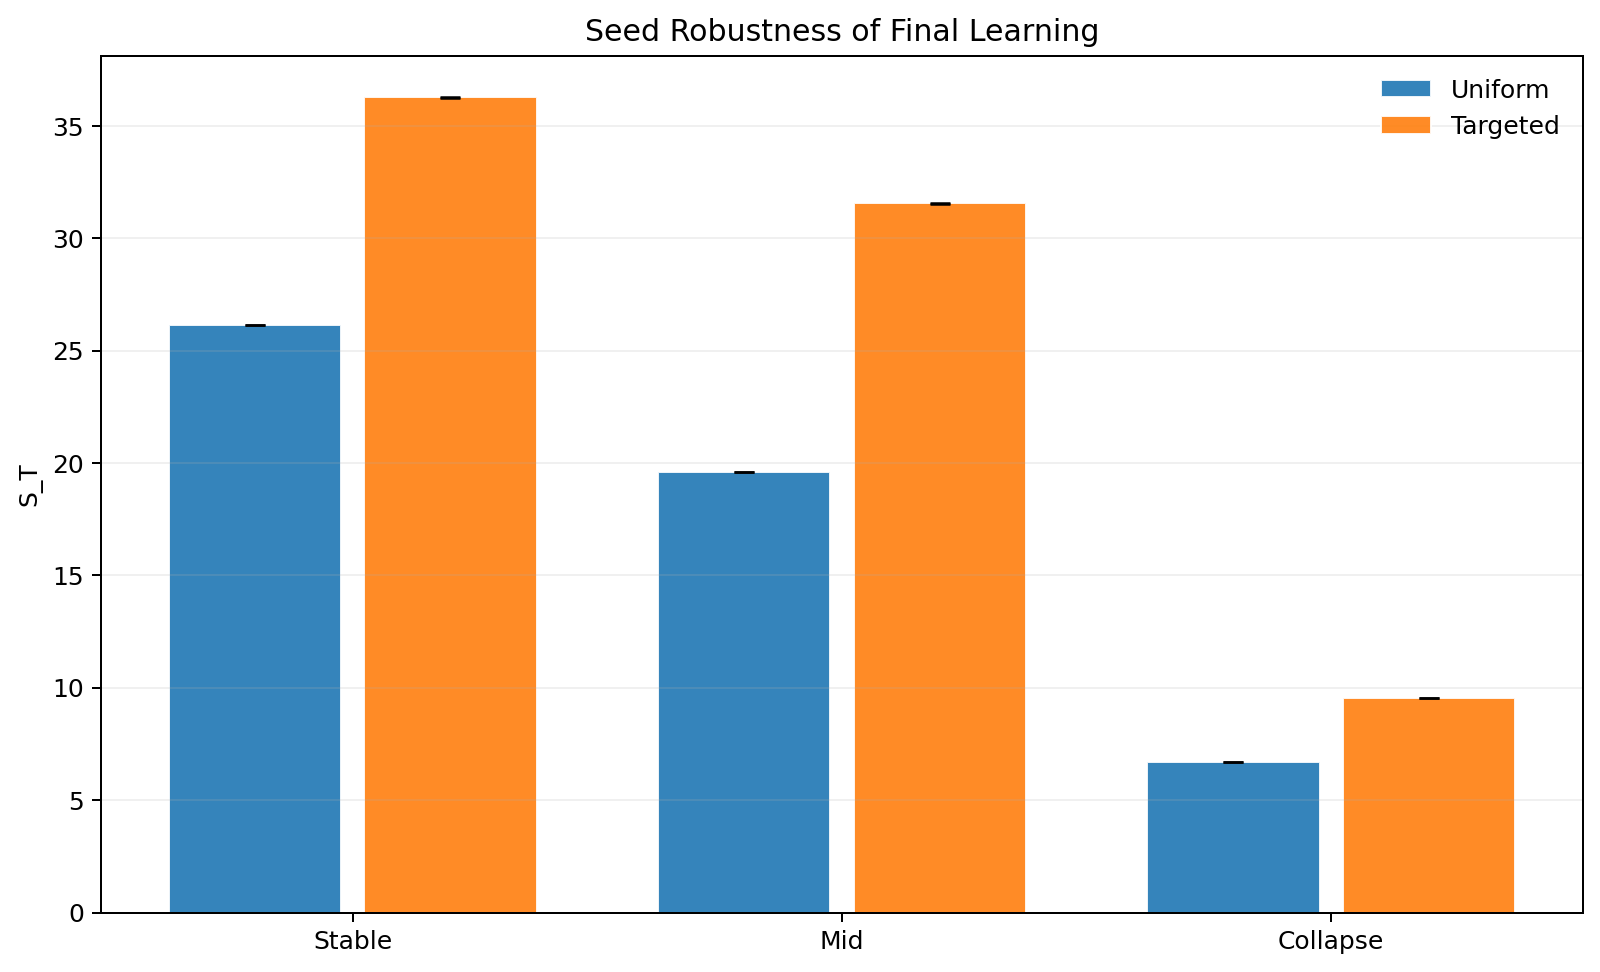
\includegraphics[width=0.48\textwidth]{../sim/figs/extra/seed_robustness_ST.png}
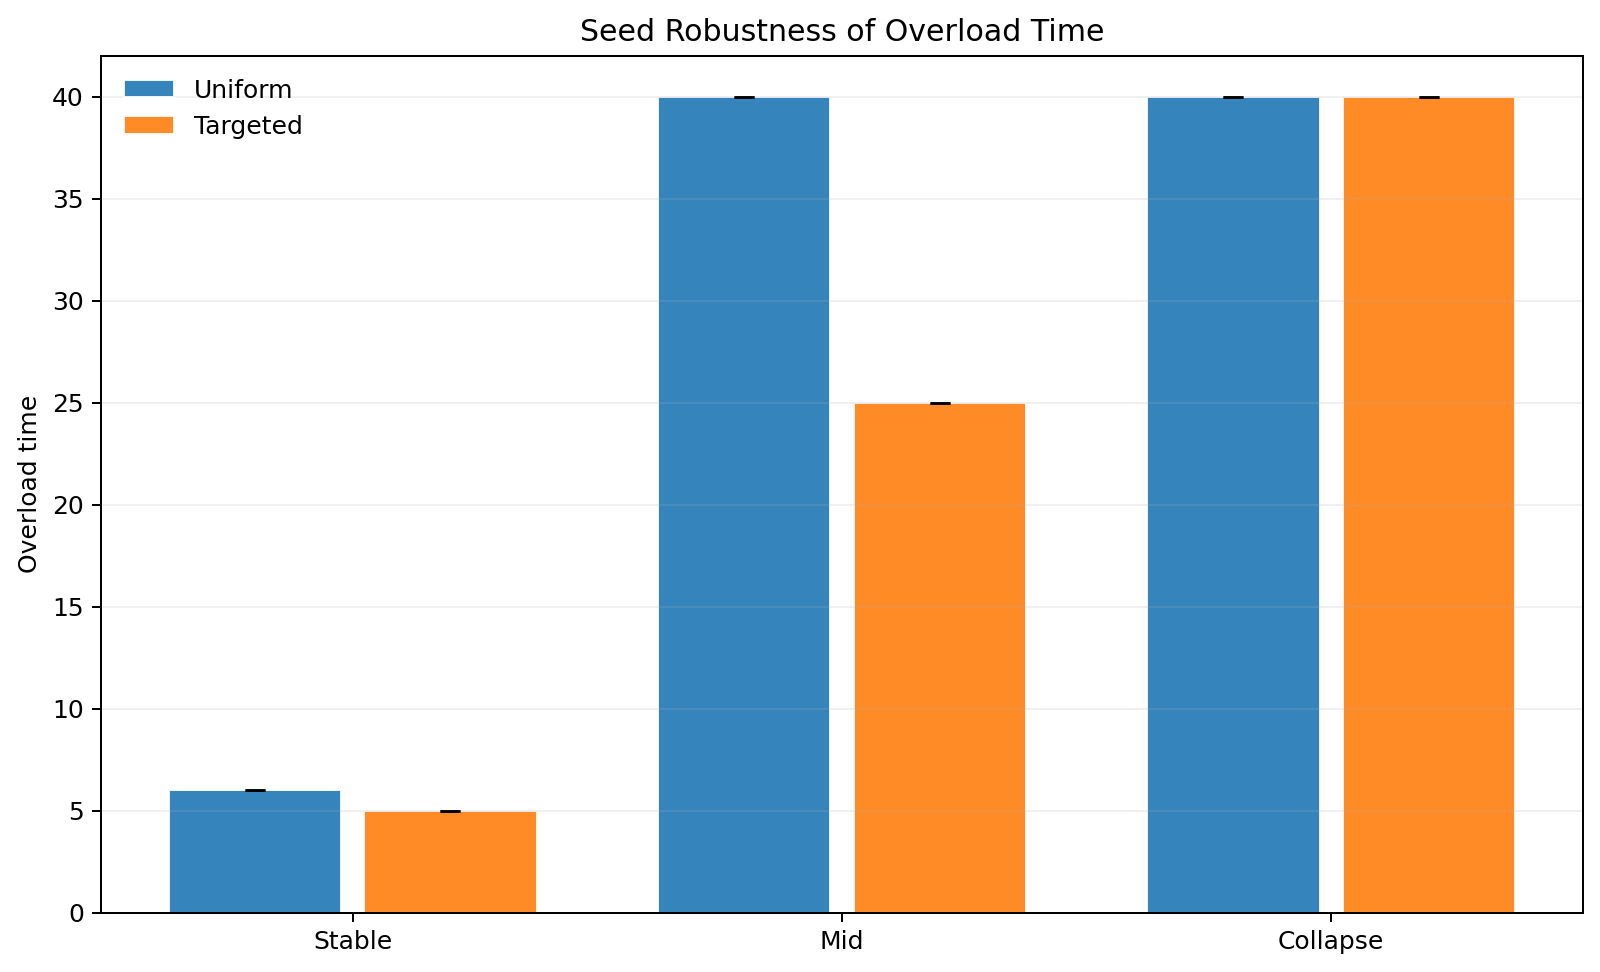
\includegraphics[width=0.48\textwidth]{../sim/figs/extra/seed_robustness_overload.png}
\caption{Seed robustness over 30 seeds. Left: final learning $S_T$. Right: overload time. The ranking is stable across novelty draws: targeted dominates uniform in stable and mid regimes and still improves learning in collapse.}
\label{fig:seed-robustness}
\end{figure}

Table~\ref{tab:extended-policy} compares four baselines in the mid regime. The capacity-aware policy improves on uniform throttling, so simple congestion feedback already has value. The stronger novelty-capacity baseline then performs even better than the targeted policy. This improves the paper's interpretation rather than weakening it: novelty-aware routing is the key ingredient, but it need not be the only one.

The comparison separates the two channels cleanly. Capacity-aware control changes \emph{how much} traffic is answered, but not \emph{which} traffic reaches the forum. Targeted deferral adds composition awareness. The novelty-capacity rule shows that composition awareness and congestion response are complementary, not competing, mechanisms.

\begin{table}[H]
\centering
\caption{Extended policy comparison in the mid regime.}
\label{tab:extended-policy}
\begin{tabular}{lrrrrr}
\toprule
Policy & $S_T$ & $\min C$ & Overload & Welfare $W$ & Revenue $U$ \\
\midrule
Uniform & 19.602 & 0.476 & 40 & 23.254 & 0.285 \\
Capacity-aware & 22.517 & 0.554 & 25 & 23.574 & 0.510 \\
Novelty+capacity & 33.232 & 0.573 & 18 & 24.894 & 0.808 \\
Targeted & 31.559 & 0.541 & 25 & 24.623 & 0.578 \\
\bottomrule
\end{tabular}
\end{table}

\begin{figure}[H]
\centering
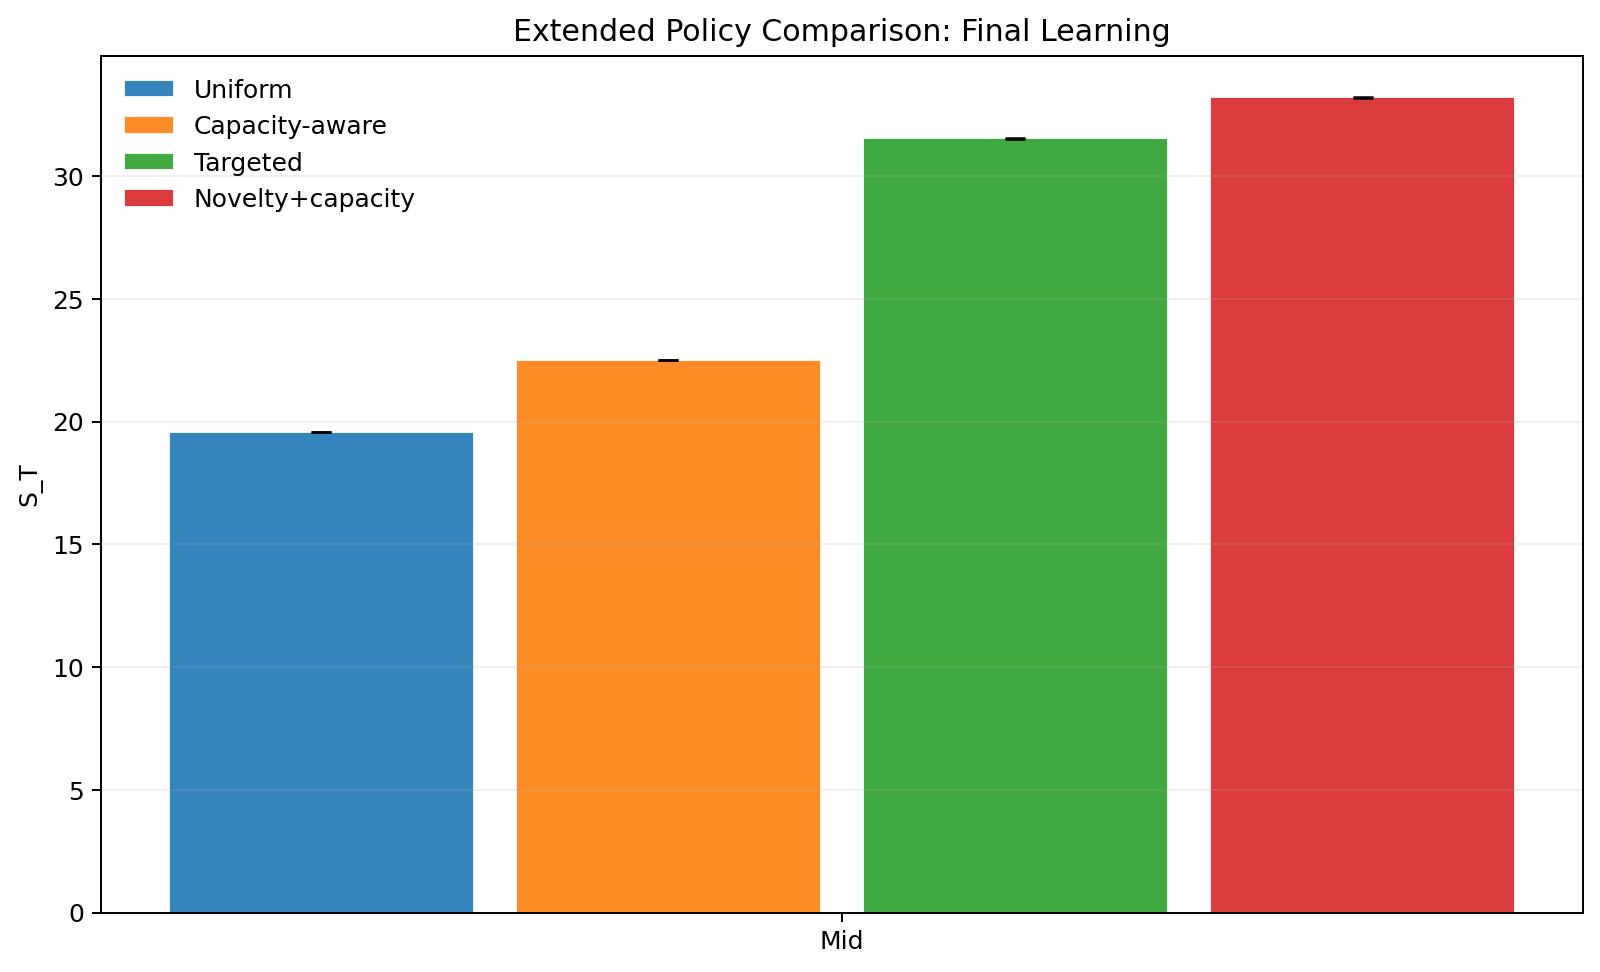
\includegraphics[width=0.48\textwidth]{../sim/figs/extra/policy_compare_extended_ST.png}
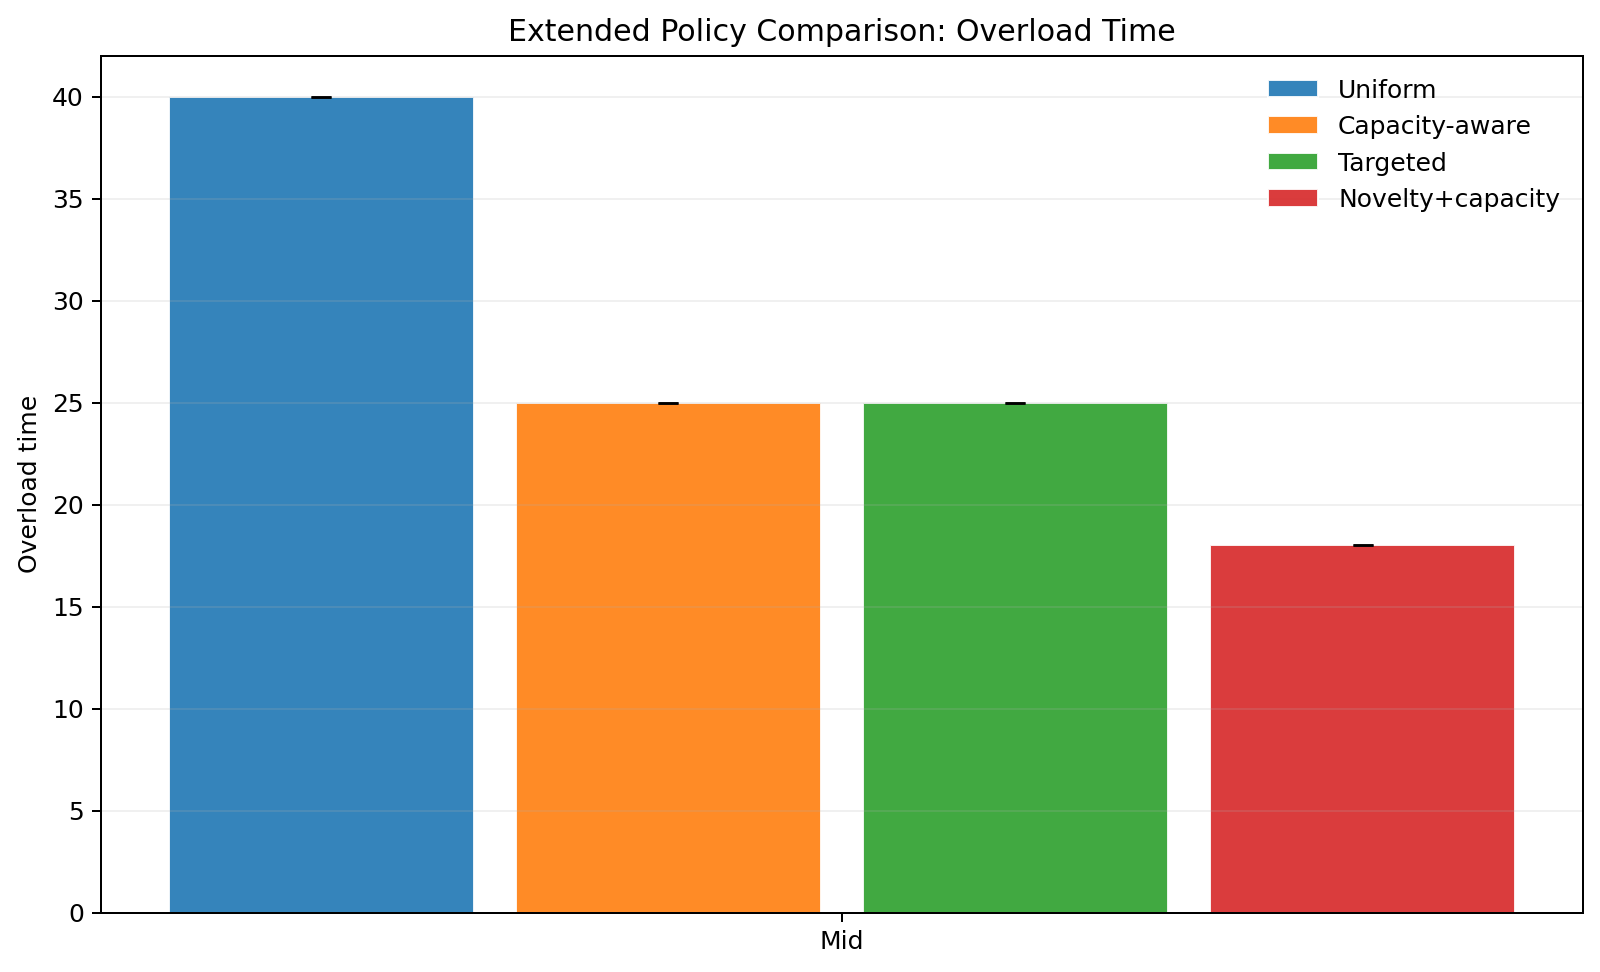
\includegraphics[width=0.48\textwidth]{../sim/figs/extra/policy_compare_extended_overload.png}
\caption{Extended policy comparison in the mid regime. Congestion response helps relative to uniform throttling, novelty awareness helps more, and the strongest rule combines both. This reinforces the paper's main message that volume and composition should be studied together.}
\label{fig:policy-compare}
\end{figure}

\subsection{Novelty Distribution Robustness}
We also checked whether the result depends on one very specific novelty distribution. The answer is no. Across four Beta distributions, targeted deferral always beats uniform throttling in final learning. The effect is largest when the deferred traffic has more high-value tail mass, but the direction is stable in all settings we tested.

\begin{table}[H]
\centering
\caption{Targeted $-$ uniform gain in $S_T$ across novelty distributions in the mid regime.}
\label{tab:novelty-dist}
\begin{tabular}{lr}
\toprule
Novelty distribution & $\Delta S_T$ \\
\midrule
Beta$(0.5,0.5)$ & 13.450 \\
Beta$(1,1)$ & 11.957 \\
Beta$(2,5)$ & 14.358 \\
Beta$(5,2)$ & 5.375 \\
\bottomrule
\end{tabular}
\end{table}

\begin{figure}[H]
\centering
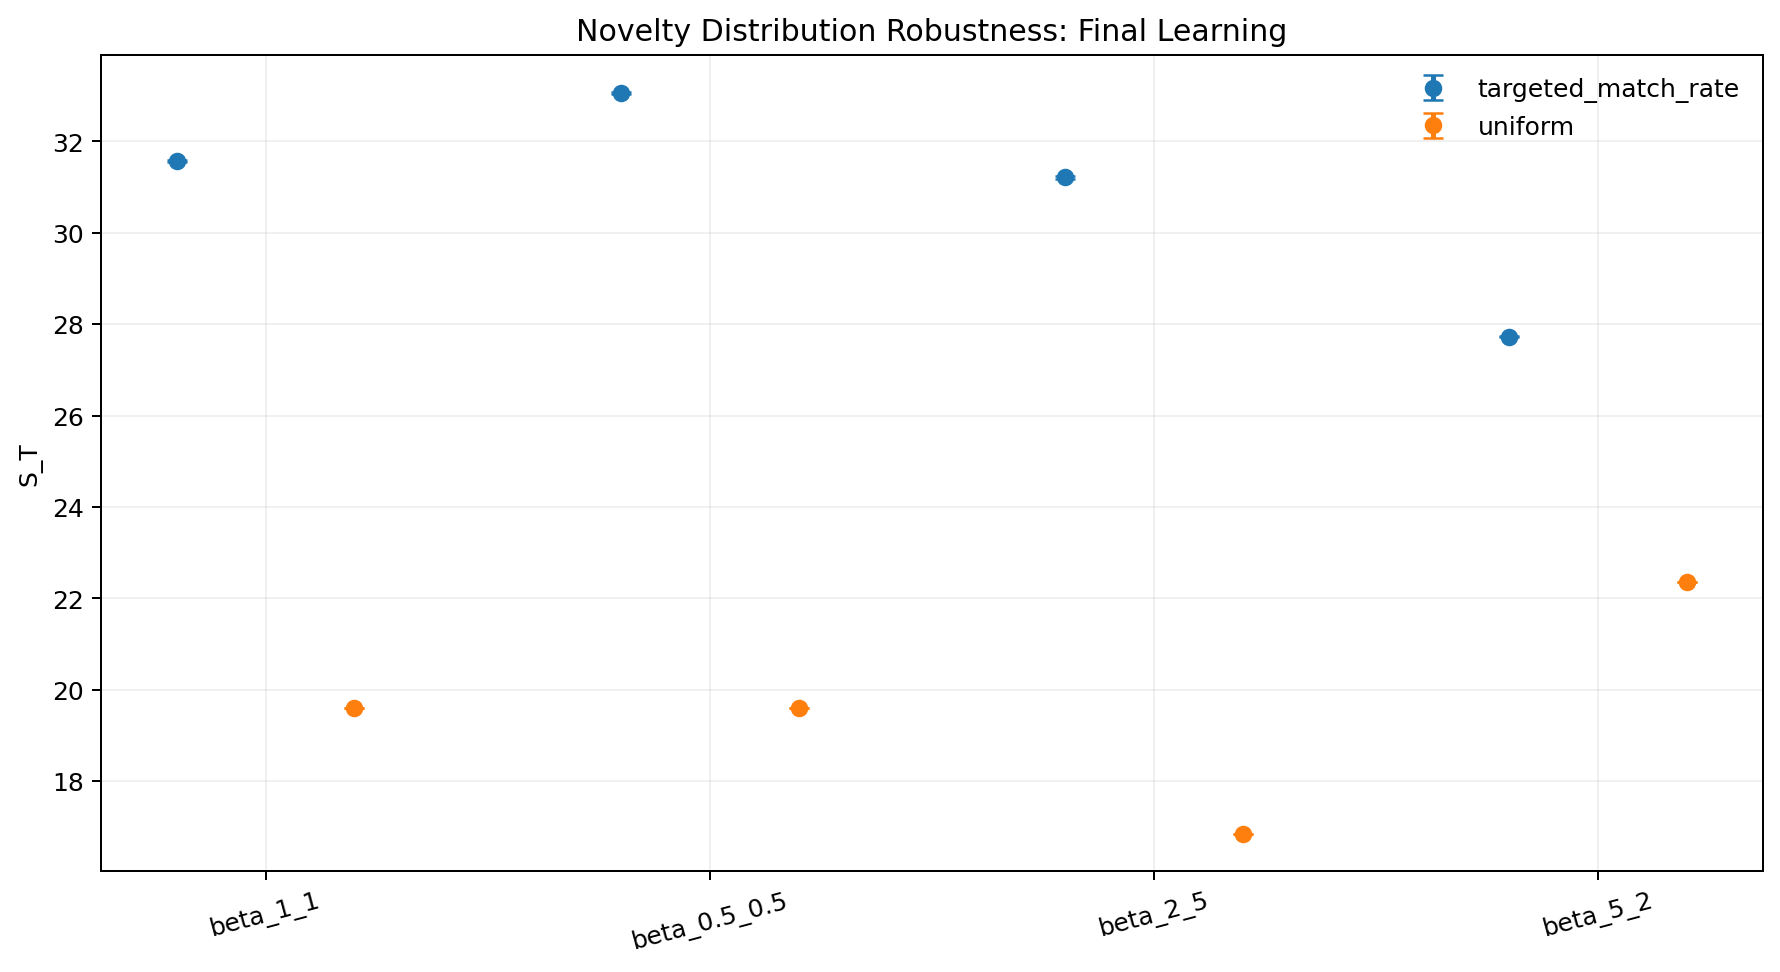
\includegraphics[width=0.48\textwidth]{../sim/figs/extra/novelty_dist_ST.png}
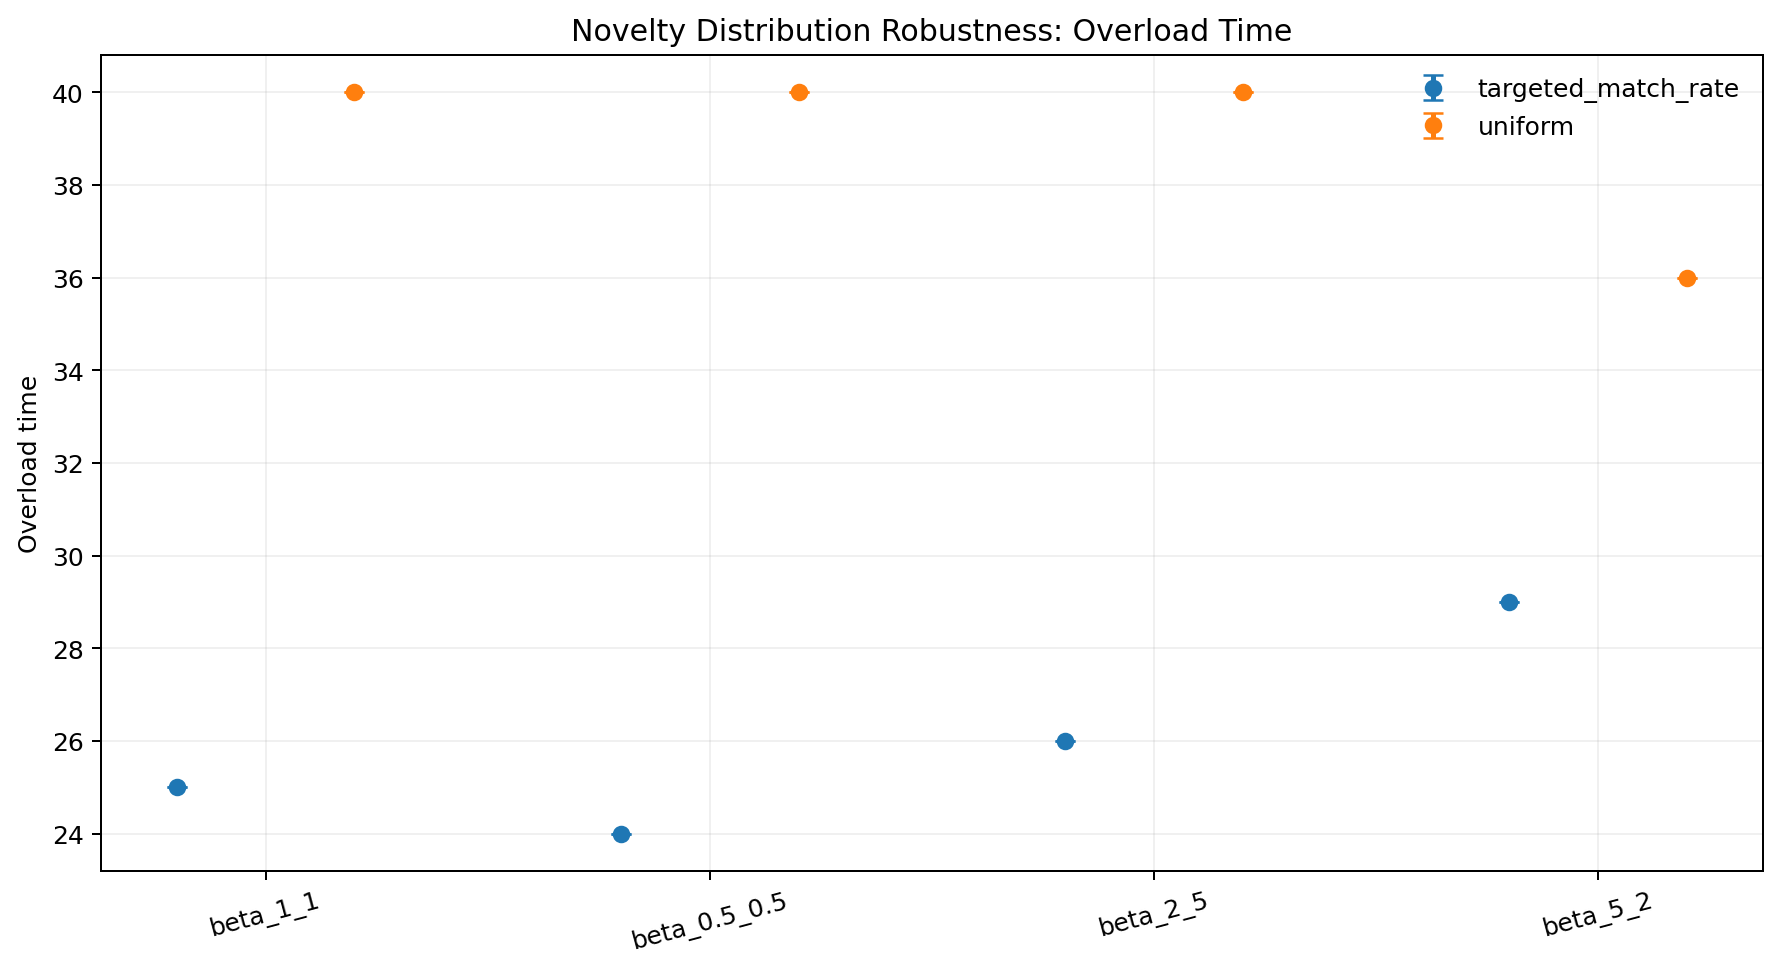
\includegraphics[width=0.48\textwidth]{../sim/figs/extra/novelty_dist_overload.png}
\caption{Novelty-distribution robustness in the mid regime. The targeted policy remains stronger than uniform even when the novelty distribution changes.}
\label{fig:novelty-dist}
\end{figure}

\section{Mechanism Validation}
The strongest mechanism check is the $\rho$ ablation. Here $\rho$ controls how strongly novelty affects the value of forum traffic. If targeted deferral is really helping by sending higher-value traffic to the forum, then its advantage should disappear when novelty does not matter.

That is exactly what we observe in Table~\ref{tab:rho}. At $\rho=0$, the targeted-uniform gap in $S_T$ is exactly $0.000$. As $\rho$ increases to $0.5$, $1.0$, and $2.0$, the gain rises to $7.228$, $11.957$, and $17.532$.

This result is unusually clean because it lines up directly with Observation 4. The gain switches off exactly when the model removes the novelty channel that targeted deferral is supposed to exploit. That is much stronger than saying the policy only works in one calibration.

\begin{table}[H]
\centering
\caption{$\rho$ ablation using the 30-seed mid-regime runs.}
\label{tab:rho}
\begin{tabular}{rrr}
\toprule
$\rho$ & $\Delta S_T$ (Targeted $-$ Uniform) & $\Delta$ Overload \\
\midrule
0.0 & 0.000 & 0 \\
0.5 & 7.228 & -9 \\
1.0 & 11.957 & -15 \\
2.0 & 17.532 & -17 \\
\bottomrule
\end{tabular}
\end{table}

\begin{figure}[H]
\centering
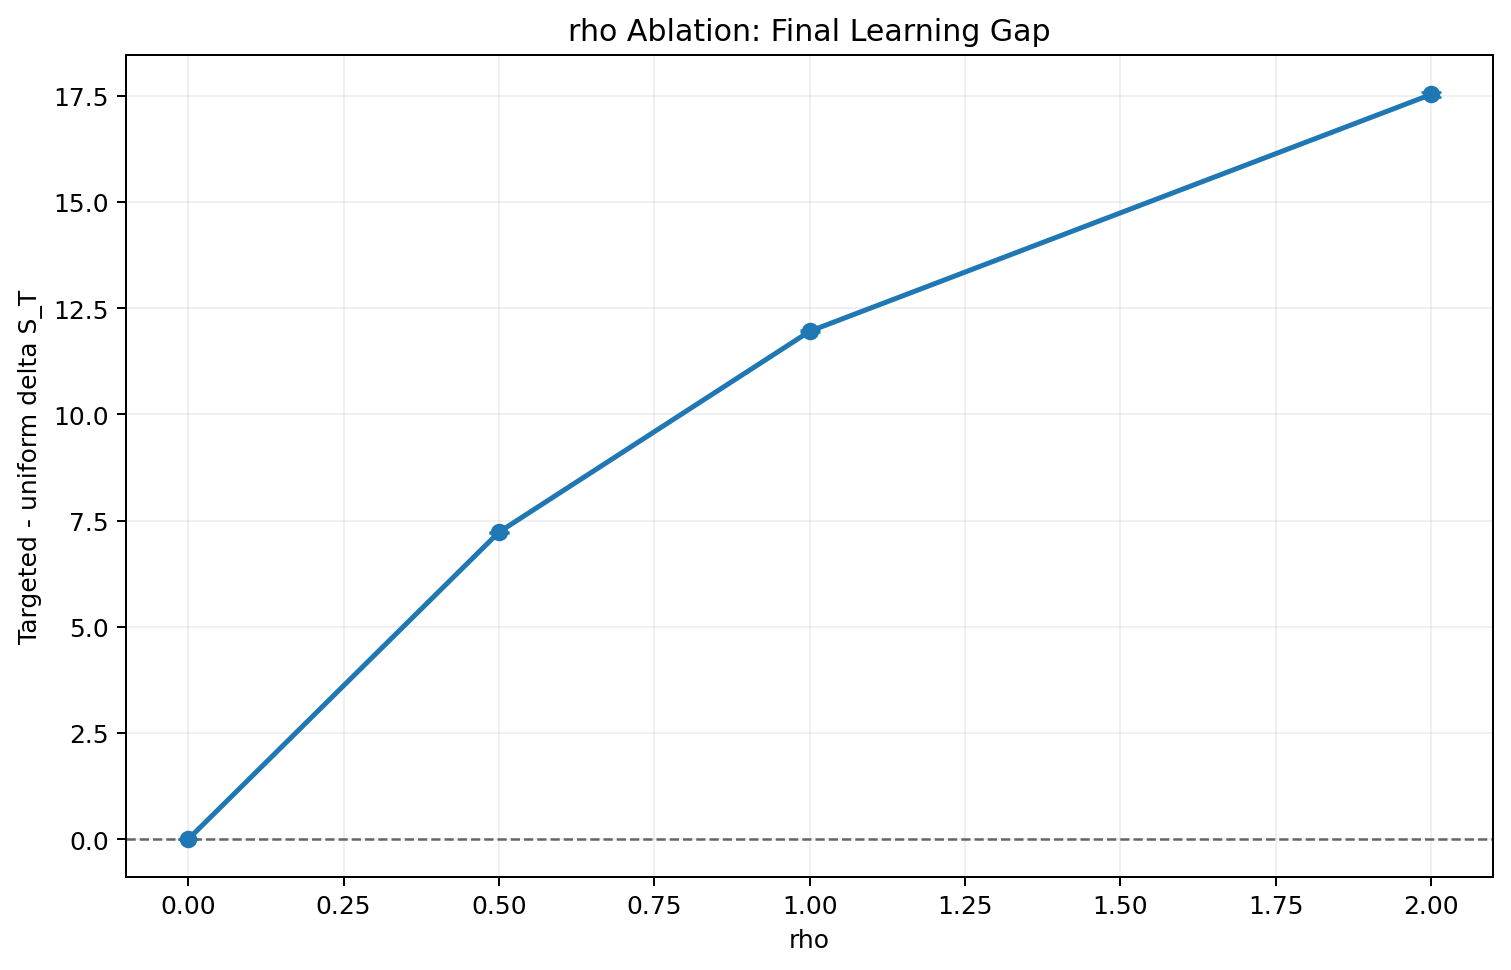
\includegraphics[width=0.48\textwidth]{../sim/figs/extra/rho_ablation_gap_ST.png}
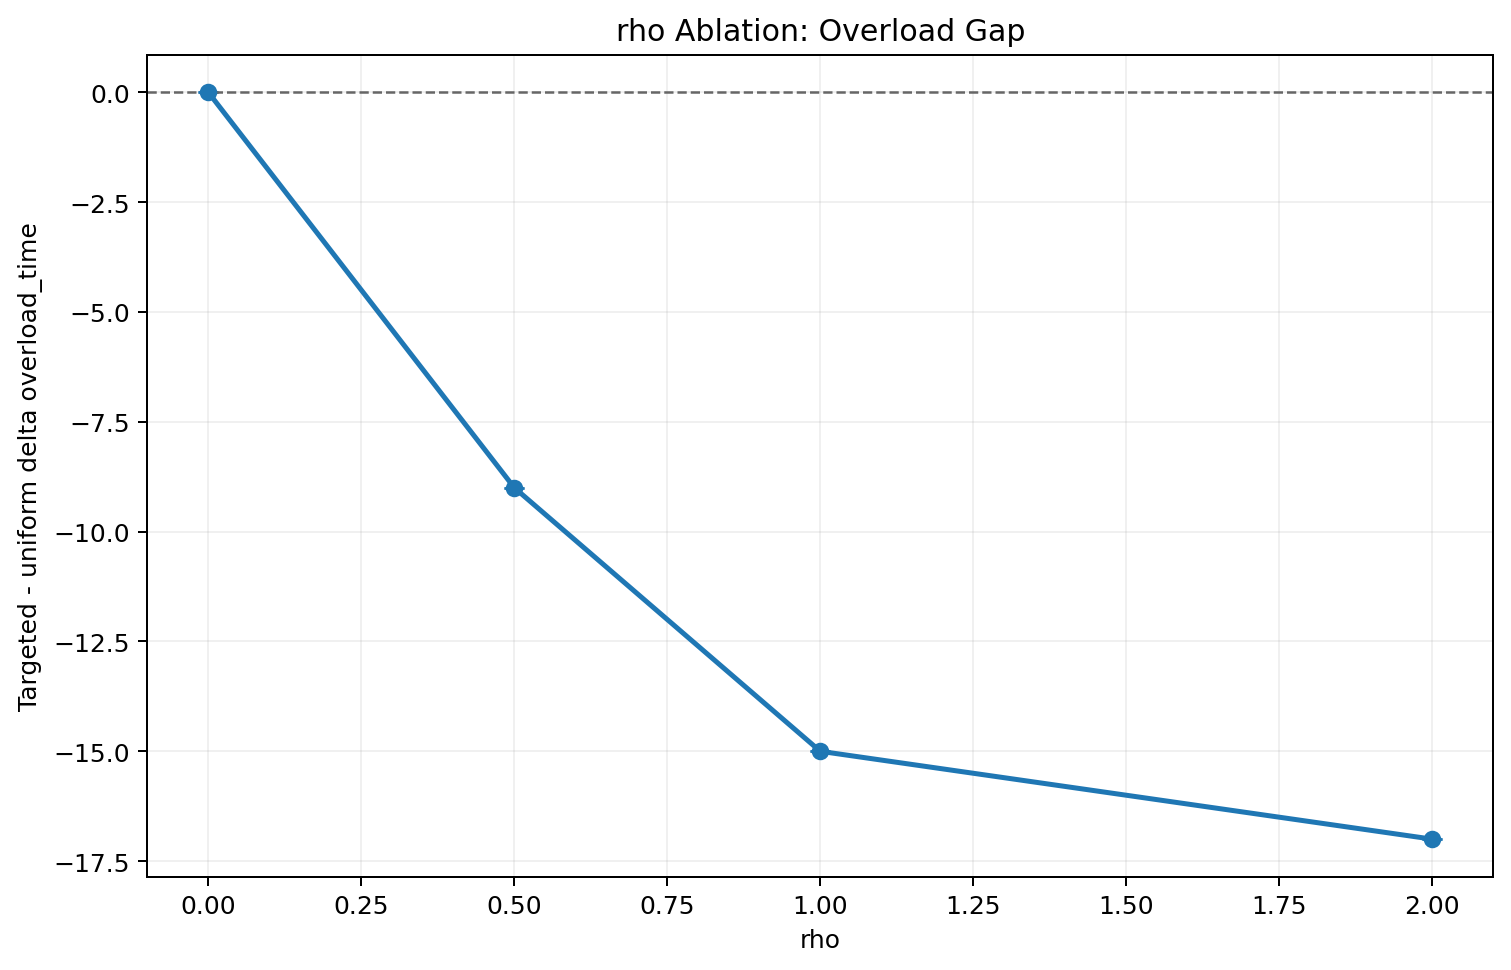
\includegraphics[width=0.48\textwidth]{../sim/figs/extra/rho_ablation_gap_overload.png}
\caption{$\rho$ ablation. When novelty has no effect ($\rho=0$), targeted deferral loses its advantage. As novelty matters more, the gain of targeted deferral grows.}
\label{fig:rho}
\end{figure}

\section{Matched Answered-Share Control}
Matching raw response rate $x$ is useful, but it does not fully control for adoption effects because $p_t^{\text{choice}}$ changes endogenously. For that reason, we added a stricter control where we tune each policy to match the actual average answered share.

The result remains strong. At matched average answered share $0.178$, the uniform policy reaches $S_T=20.585$, while the targeted policy reaches $S_T=31.349$. Overload also improves from $33$ to $30$. This means the targeted gain is not only coming from answering a larger total share of users.

This control is important for interpretation. Without it, one could argue that targeted deferral wins only because it indirectly changes adoption and answered volume. The matched-answered experiment removes that explanation. Once actual answered share is held fixed, the remaining gap is best understood as a composition effect.

\begin{table}[H]
\centering
\caption{Matched answered-share control in the mid regime.}
\label{tab:matched-answered}
\begin{tabular}{lrrrr}
\toprule
Policy & Avg. answered & Avg. answer rate & $S_T$ & Overload \\
\midrule
Uniform matched answered & 0.178 & 0.631 & 20.585 & 33 \\
Targeted matched answered & 0.178 & 0.574 & 31.349 & 30 \\
\bottomrule
\end{tabular}
\end{table}

\begin{figure}[H]
\centering
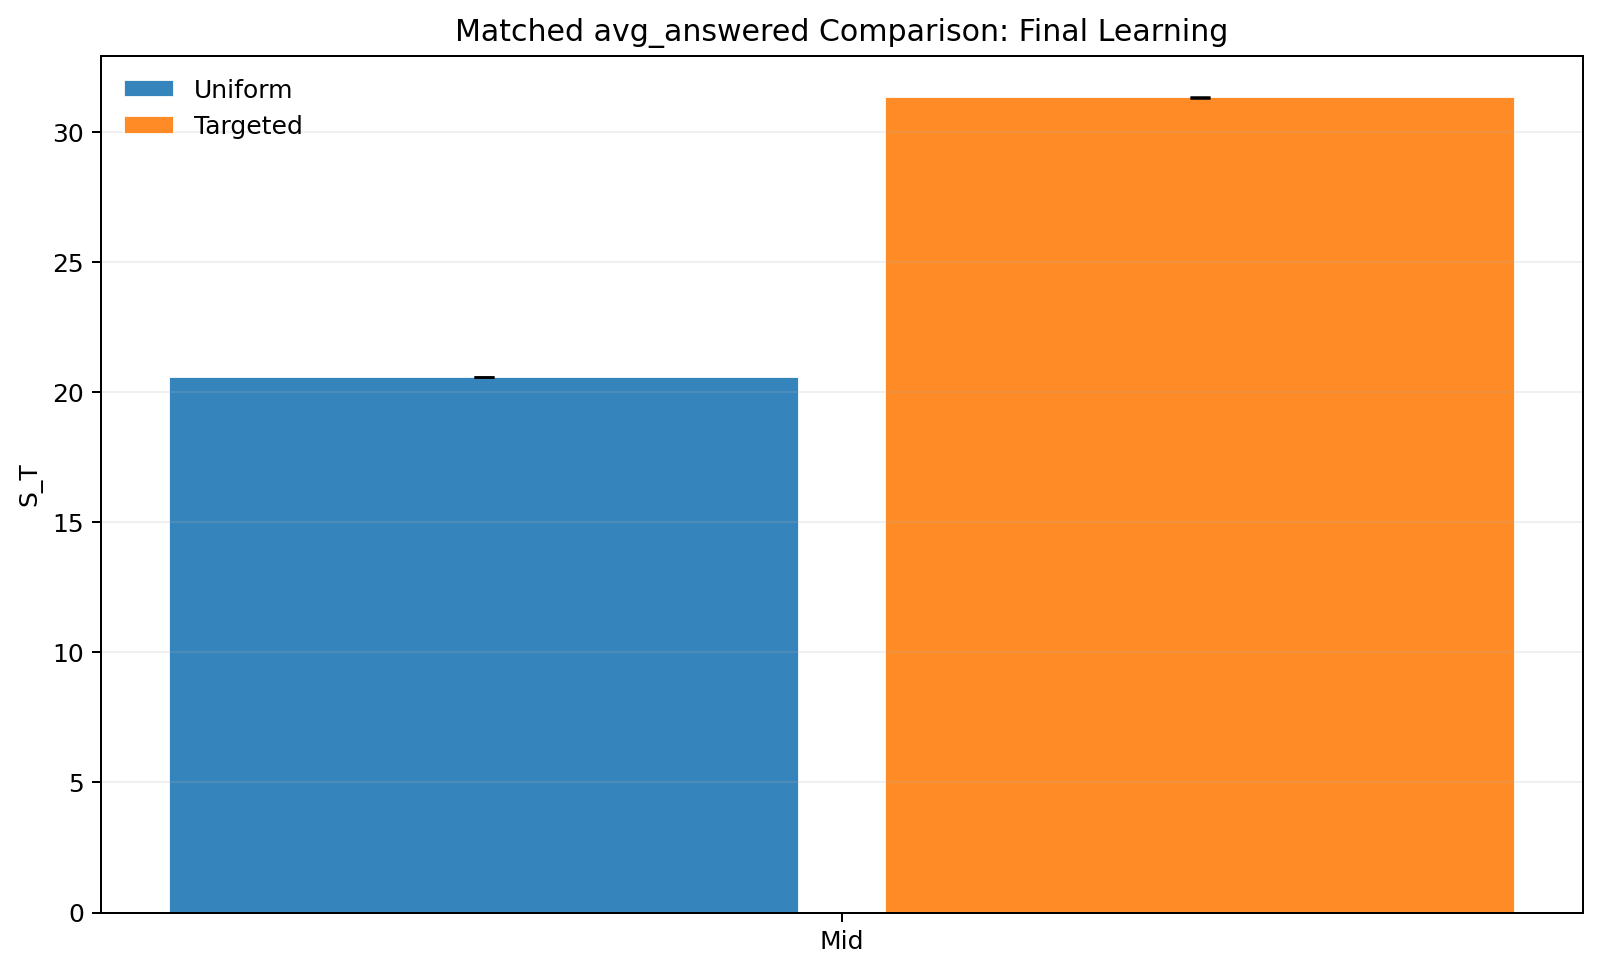
\includegraphics[width=0.62\textwidth]{../sim/figs/extra/matched_answered_compare_ST.png}
\caption{Matched answered-share comparison. Even after tuning the two policies so that actual answered share is the same, targeted deferral keeps a large learning advantage.}
\label{fig:matched-answered}
\end{figure}

\section{Tipping Boundary and Phase Transition}
The heatmaps show that collapse is not random. It appears in a structured region of parameter space. To make this clear, we extracted a binary collapse mask using the rule $\min_t C_t < 0.05$ and plotted the boundary in the $(C_1,\xi)$ plane.

The first collapse points appear around $C_1 \approx 0.364$ and $\xi \approx 0.074$. As $\xi$ increases, the system needs a larger initial capacity to stay healthy. This is the clearest phase-transition picture in our simulator.

At the same time, the boundary should be read carefully. It is a threshold map built from a finite parameter grid, a fixed horizon $T=40$, and the rule $\min_t C_t < 0.05$. So the slightly step-like shape in Figure~\ref{fig:collapse-boundary} partly reflects discretization and threshold choice, not an exact closed-form phase line. The important point is qualitative: there is a clear region where overload damage begins to dominate replenishment, and that region moves in the expected direction as $C_1$ and $\xi$ change.

\begin{figure}[H]
\centering
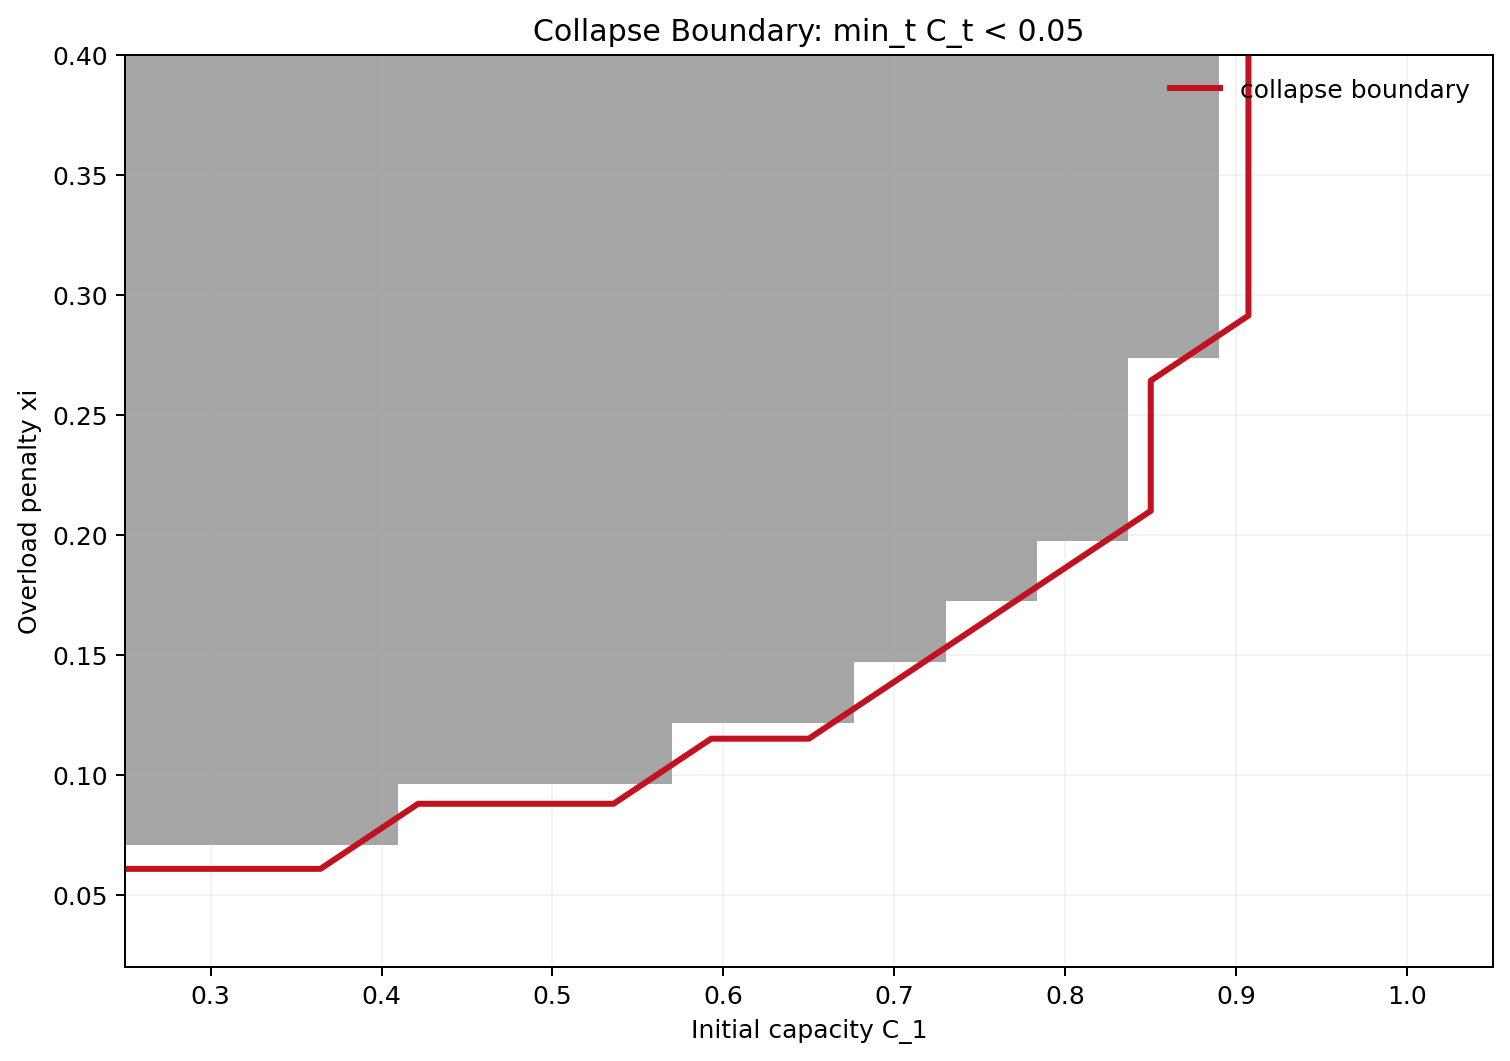
\includegraphics[width=0.60\textwidth]{../sim/figs/extra/collapse_boundary_c1_xi.png}
\caption{Explicit collapse boundary in the $(C_1,\xi)$ plane using the rule $\min_t C_t < 0.05$. Higher overload penalties push the system into collapse unless the initial forum capacity is sufficiently large.}
\label{fig:collapse-boundary}
\end{figure}

\begin{figure}[H]
\centering
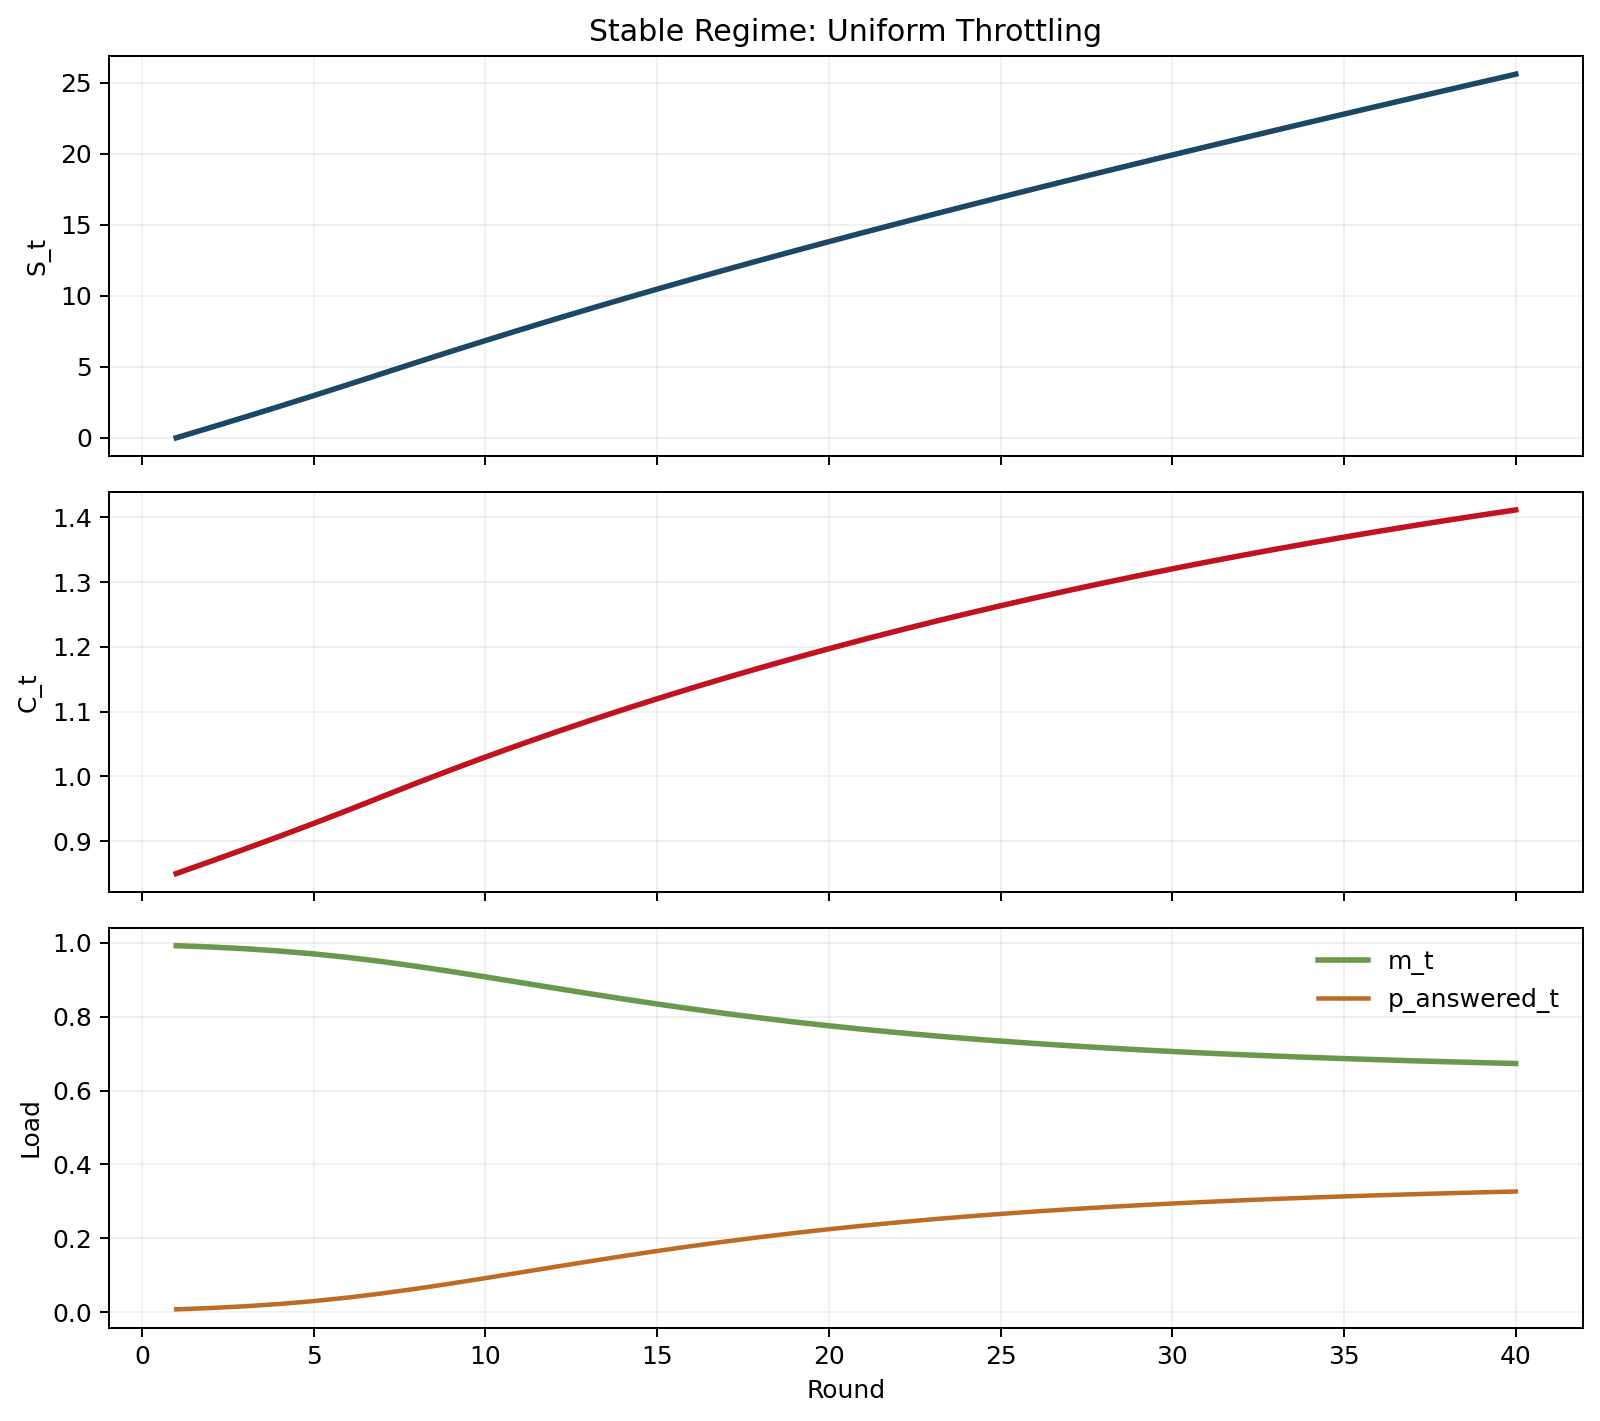
\includegraphics[width=0.48\textwidth]{../sim/figs/timeseries_stable.png}
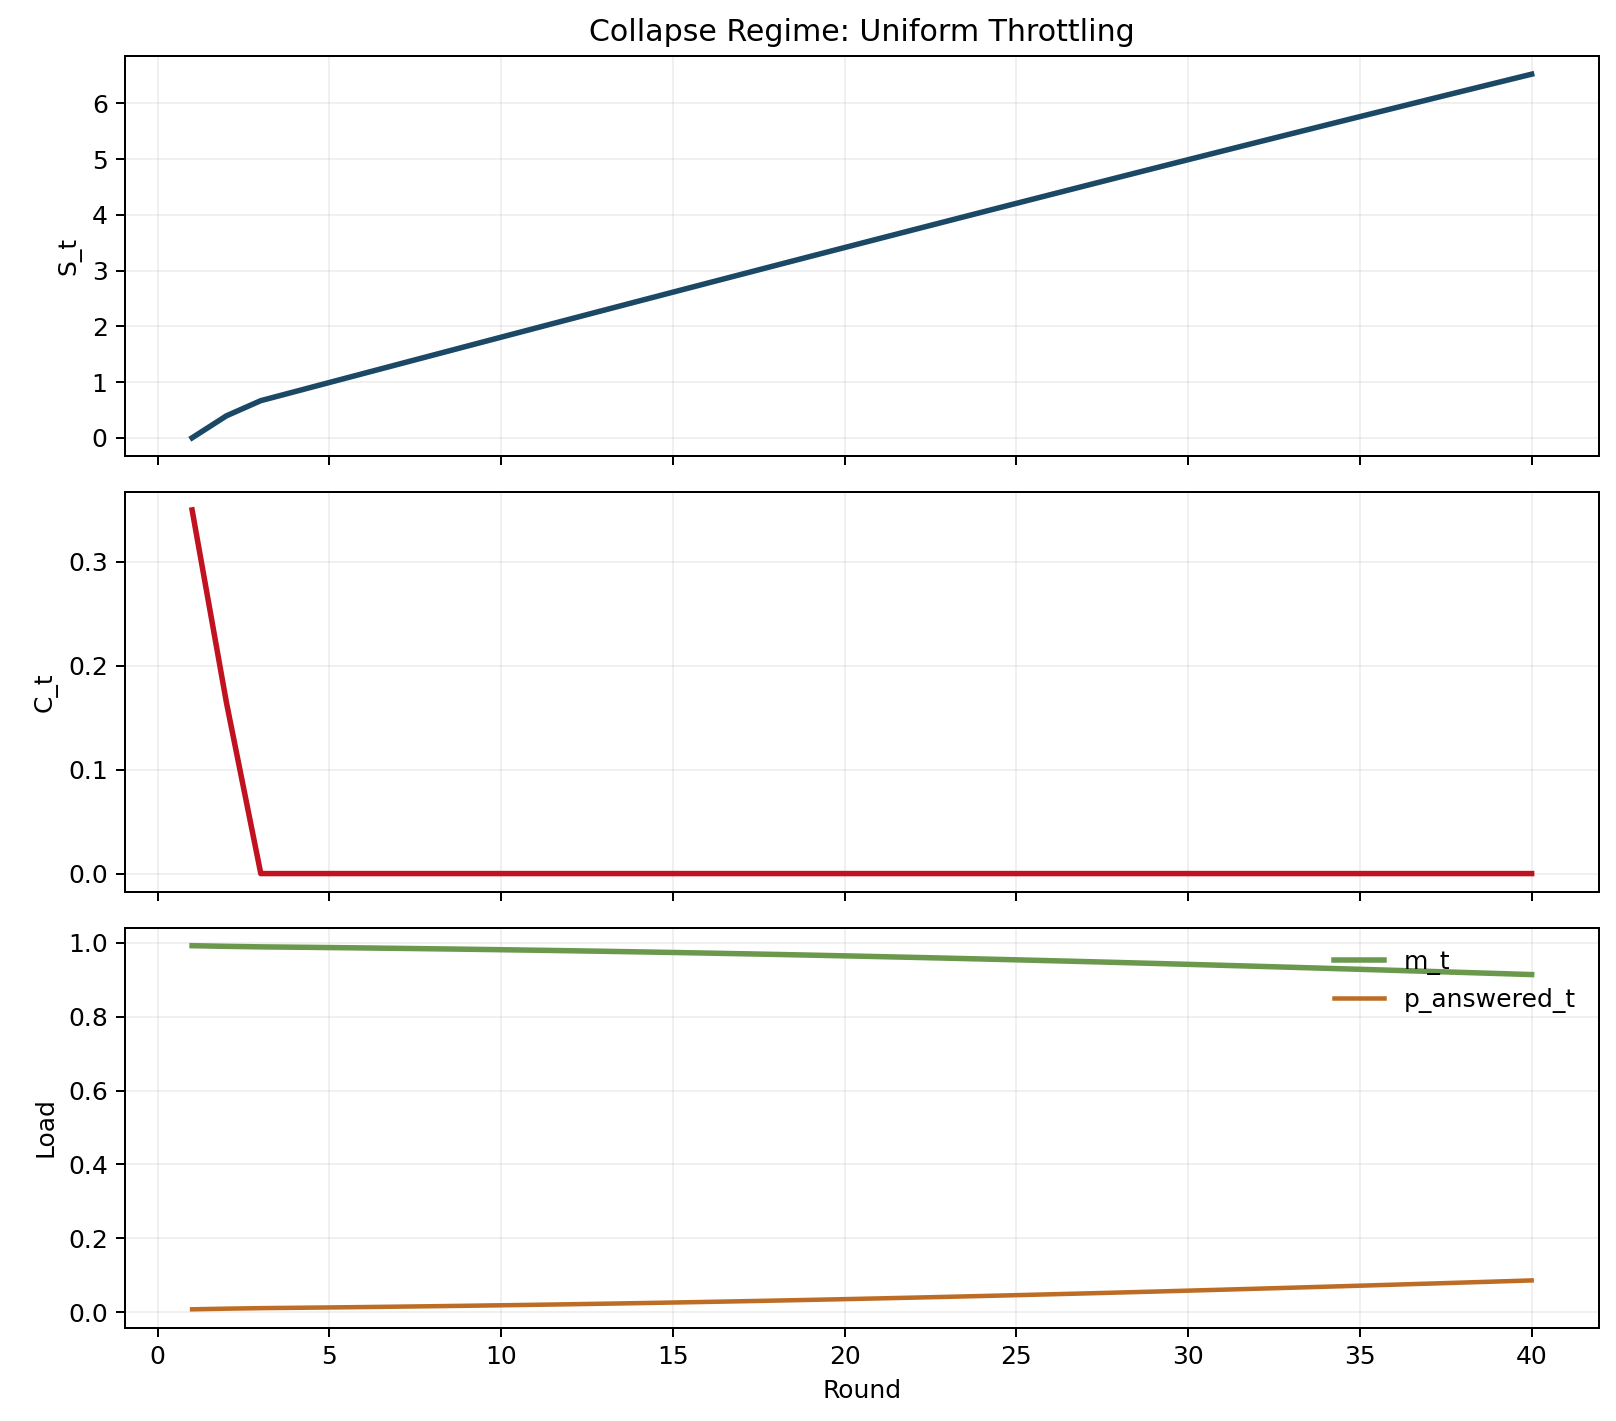
\includegraphics[width=0.48\textwidth]{../sim/figs/timeseries_collapse.png}
\caption{Time-series examples. Left: stable regime, where capacity remains healthy and knowledge grows steadily. Right: collapse regime, where overload damages capacity and the system falls into a bad state.}
\label{fig:timeseries}
\end{figure}

\section{Discussion}
The results support a simple story. Uniform throttling is too blunt. It can reduce load, but it does not control which traffic reaches the forum. Capacity-aware control is better because it reacts to congestion, but it still does not separate high-value forum traffic from low-value forum traffic.

The core advantage comes from novelty-aware routing. The targeted policy is the simplest rule that uses this idea directly: it sends traffic with higher knowledge value to the forum while still keeping total forum pressure under control in many regimes. In the model, that means it improves the novelty factor without requiring a proportionate increase in productive load. The matched answered-share control is important here, because it shows the gain is not only from changing adoption levels.

The collapse regime also teaches a limit. Once the system is deep in overload, selective response cannot fully rescue it. In that case, the forum is already too damaged, and policy improvements mainly recover some learning, not forum health. This is exactly what the capacity equation predicts: once overload repeatedly reduces future capacity, a better routing policy may help on the margin but cannot undo a badly degraded state immediately.

Another important lesson is that learning is not the only objective in the simulator. The paper also reports a welfare proxy $W$ and a revenue proxy $U$, and the $x$-sweep plots show that these objectives do not peak at the same answer rate as $S_T$. That mismatch matters. A planner who only values long-run learning may choose a different policy than a planner who prioritizes short-run welfare, revenue, or forum preservation. This is one reason the paper should be read as an ecosystem study rather than a single-objective optimization claim.

More broadly, the paper suggests a two-part lesson. First, answering policy should be evaluated as part of a larger ecosystem, not only as a one-shot service decision. Second, when the external human channel is congestible, composition can matter just as much as volume.

\section{Implementation Notes and Sanity Checks}
While building the simulator, we used several checks to make sure the results were not an artifact of one configuration. First, we ran both quick and full modes and verified that the large-scale findings were almost unchanged. Second, we added the matched answered-share control because matching only the raw answer rate can be misleading once user adoption shifts. Third, we added the $\rho=0$ ablation to test the mechanism directly.

We also checked whether a simple congestion-reactive policy could explain the gain. It could not. The capacity-aware baseline helps, but it does not match the novelty-aware policies. The stronger novelty-capacity baseline then shows that adding congestion response on top of novelty routing can improve performance further. This matters because the result is not simply ``answer more when overloaded.'' Traffic composition matters, and it can be combined with congestion feedback.

\begin{designchoice}
We treated mechanism validation as a required part of the project rather than a bonus plot. Without the $\rho=0$ test and the matched answered-share control, it would be much harder to argue that the targeted advantage is real.
\end{designchoice}

\section{Limitations}
Our model is intentionally small. It uses a reduced-form knowledge stock and a reduced-form capacity process. It does not model explicit posts, expert heterogeneity, retraining lags, or user churn.

The novelty weighting is also stylized. We treat novelty as a Beta-distributed score and summarize its contribution through a single parameter $\rho$. This is useful for mechanism testing, but it is still an abstraction.

Finally, the current simulator treats one forum and one GenAI channel. Real systems often involve multiple communities, cross-posting, search effects, and delayed data collection. For that reason, all of the empirical claims in this paper should be read as claims within this reduced-form simulator, not as direct claims about any one real platform.

\section{Conclusion and Future Work}
This report extends selective response with forum congestion and endogenous capacity. The model is intentionally reduced-form, but that simplicity is a feature rather than a weakness for the question we study. It lets us isolate a small number of forces and see how they interact.

The main result is clear: novelty-aware routing improves long-run learning relative to uniform throttling in this reduced-form simulator, and in healthy or middle regimes it can also reduce overload. The mechanism check is especially strong because the targeted advantage disappears when novelty is set to have no effect. The matched answered-share control also shows that the gain is not only a byproduct of higher effective service volume. At the same time, the stronger novelty-capacity baseline shows that congestion response and novelty-aware routing can be combined, and in the extended mid-regime comparison that hybrid rule performs best. So the paper should not be read as claiming that one fixed hand-designed rule is universally optimal.

There are several natural next steps. A richer model could include explicit forum churn, retraining delays, and multi-platform competition. Another useful extension would be a budgeted policy that jointly optimizes user welfare, revenue, and forum health. Finally, it would be interesting to connect the simulator to real traces from public technical forums.

\appendix

\section{Appendix Overview}
This appendix consolidates the settings, robustness summaries, and extra plots that support the main text. The goal is to keep the body readable while still making the submission reproducible from the repository artifacts.

\section{Core Parameter Settings}
Table~\ref{tab:appendix-params} summarizes the default simulator parameters used unless an experiment explicitly varies them.

\begin{table}[H]
\centering
\caption{Default simulator parameters used across the main experiments.}
\label{tab:appendix-params}
\begin{tabular}{ll}
\toprule
Parameter & Value \\
\midrule
Horizon $T$ & 40 \\
Initial knowledge $S_1$ & 0.0 \\
Stable initial capacity $C_1$ & 0.85 \\
Mid initial capacity $C_1$ & 0.60 \\
Collapse initial capacity $C_1$ & 0.35 \\
Learning slope $\alpha$ & 0.12 \\
Choice sharpness $\beta$ & 8.0 \\
Forum utility weight $w_s$ & 0.55 \\
Knowledge scale $\kappa$ & 1.0 \\
Overflow discount $\lambda$ & 0.2 \\
Capacity decay $\delta$ & 0.03 \\
Capacity replenishment $\eta$ & 0.05 \\
Mid-regime overload penalty $\xi$ & 0.10 \\
Stable overload penalty $\xi$ & 0.04 \\
Collapse overload penalty $\xi$ & 0.35 \\
Response effort & 1.0 \\
Novelty weight & 0.35 \\
Default novelty exponent $\rho$ & 1.0 \\
Revenue discount $\gamma$ & 0.95 \\
\bottomrule
\end{tabular}
\end{table}

\section{Additional Robustness Tables}
Table~\ref{tab:appendix-novelty-full} reports the novelty-distribution robustness results in fuller form than the main-text delta summary. The targeted policy remains stronger than uniform across all four distributions, but the size of the gain depends on how much mass the novelty distribution places on forum-valuable traffic.

\begin{table}[H]
\centering
\caption{Novelty-distribution robustness in the mid regime.}
\label{tab:appendix-novelty-full}
\begin{tabular}{lrrrr}
\toprule
Distribution & Policy & $S_T$ & Overload & Avg. forum novelty \\
\midrule
Beta$(0.5,0.5)$ & Uniform & 19.602 & 40 & 0.500 \\
Beta$(0.5,0.5)$ & Targeted & 33.052 & 24 & 0.878 \\
Beta$(1,1)$ & Uniform & 19.602 & 40 & 0.500 \\
Beta$(1,1)$ & Targeted & 31.559 & 25 & 0.800 \\
Beta$(2,5)$ & Uniform & 16.852 & 40 & 0.286 \\
Beta$(2,5)$ & Targeted & 31.210 & 26 & 0.447 \\
Beta$(5,2)$ & Uniform & 22.350 & 36 & 0.714 \\
Beta$(5,2)$ & Targeted & 27.725 & 29 & 0.865 \\
\bottomrule
\end{tabular}
\end{table}

Table~\ref{tab:appendix-rho-full} expands the $\rho$ ablation by reporting the policy levels rather than only the targeted-minus-uniform gap. This makes it clear that the composition advantage disappears exactly when novelty stops affecting knowledge production.

\begin{table}[H]
\centering
\caption{Full $\rho$ ablation in the mid regime.}
\label{tab:appendix-rho-full}
\begin{tabular}{lrrrr}
\toprule
$\rho$ & Policy & $S_T$ & Overload & Avg. novelty factor \\
\midrule
0.0 & Uniform & 25.543 & 31 & 1.000 \\
0.0 & Targeted & 25.543 & 31 & 1.000 \\
0.5 & Uniform & 21.774 & 37 & 0.883 \\
0.5 & Targeted & 29.002 & 28 & 1.118 \\
1.0 & Uniform & 19.602 & 40 & 0.825 \\
1.0 & Targeted & 31.559 & 25 & 1.210 \\
2.0 & Uniform & 17.446 & 40 & 0.767 \\
2.0 & Targeted & 34.978 & 23 & 1.336 \\
\bottomrule
\end{tabular}
\end{table}

Table~\ref{tab:appendix-matched-full} gives the fuller matched answered-share comparison. The two policies are tuned to the same average answered share, so the remaining learning gap should be read as a composition effect rather than a raw service-volume effect.

\begin{table}[H]
\centering
\small
\caption{Full matched answered-share comparison in the mid regime.}
\label{tab:appendix-matched-full}
\begin{tabular}{lrrrrr}
\toprule
Policy & Avg. answered & Avg. answer rate & $S_T$ & Overload & Avg. forum novelty \\
\midrule
Uniform matched answered & 0.178 & 0.631 & 20.585 & 33 & 0.500 \\
Targeted matched answered & 0.178 & 0.574 & 31.349 & 30 & 0.787 \\
\bottomrule
\end{tabular}
\end{table}

\section{Additional Plots}
The figures below collect the extra plots used for diagnostics and robustness checks.

\begin{figure}[H]
\centering
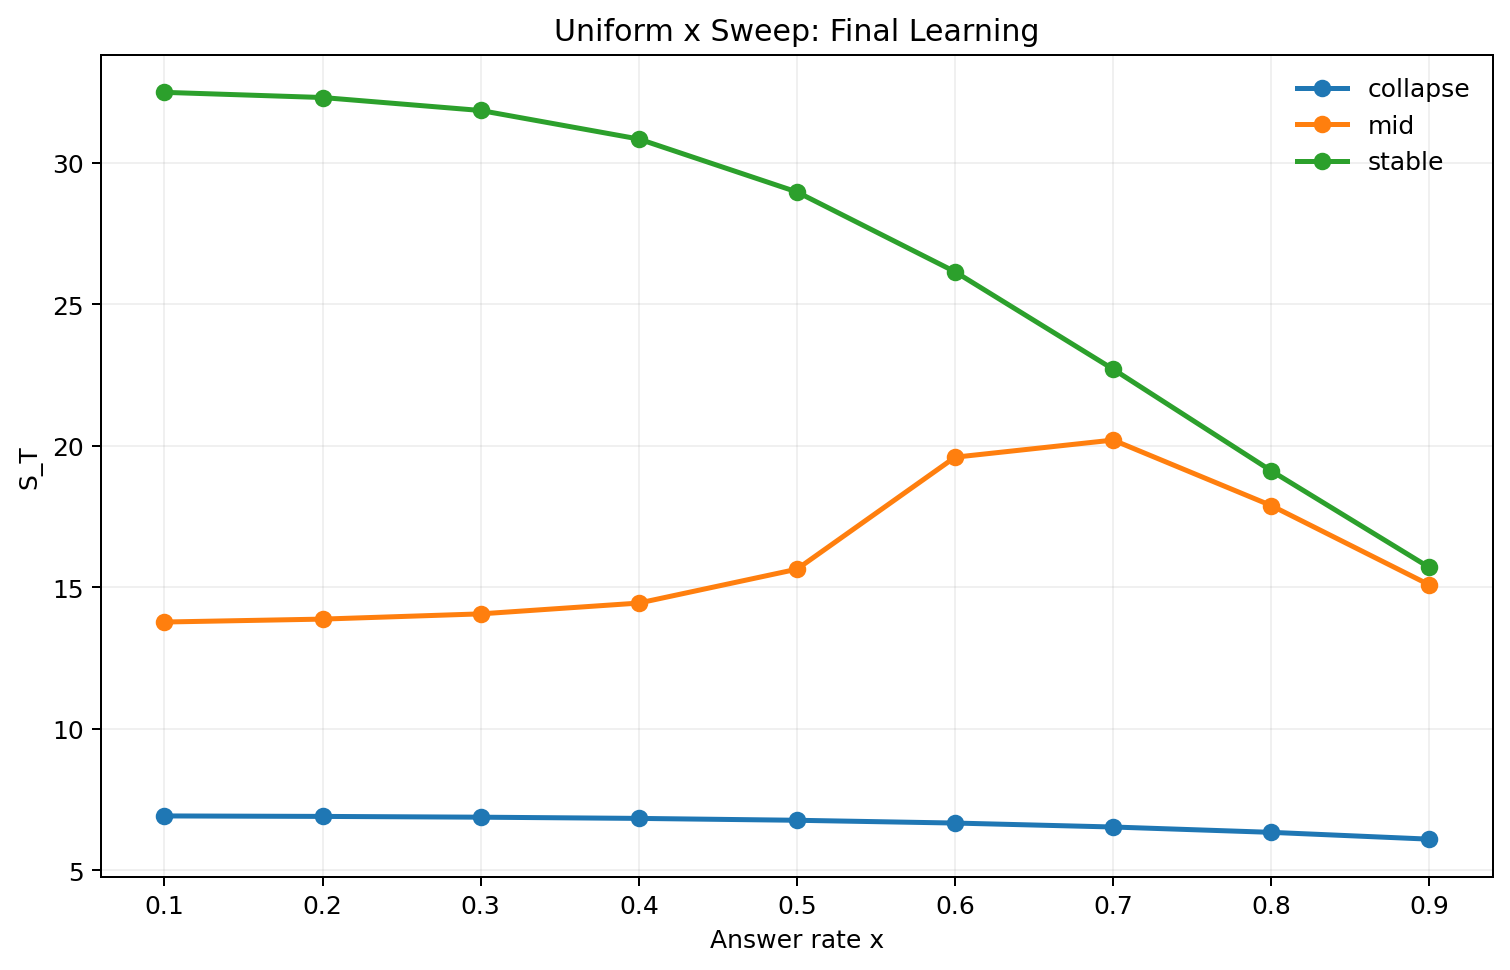
\includegraphics[width=0.48\textwidth]{../sim/figs/extra/x_sweep_ST.png}
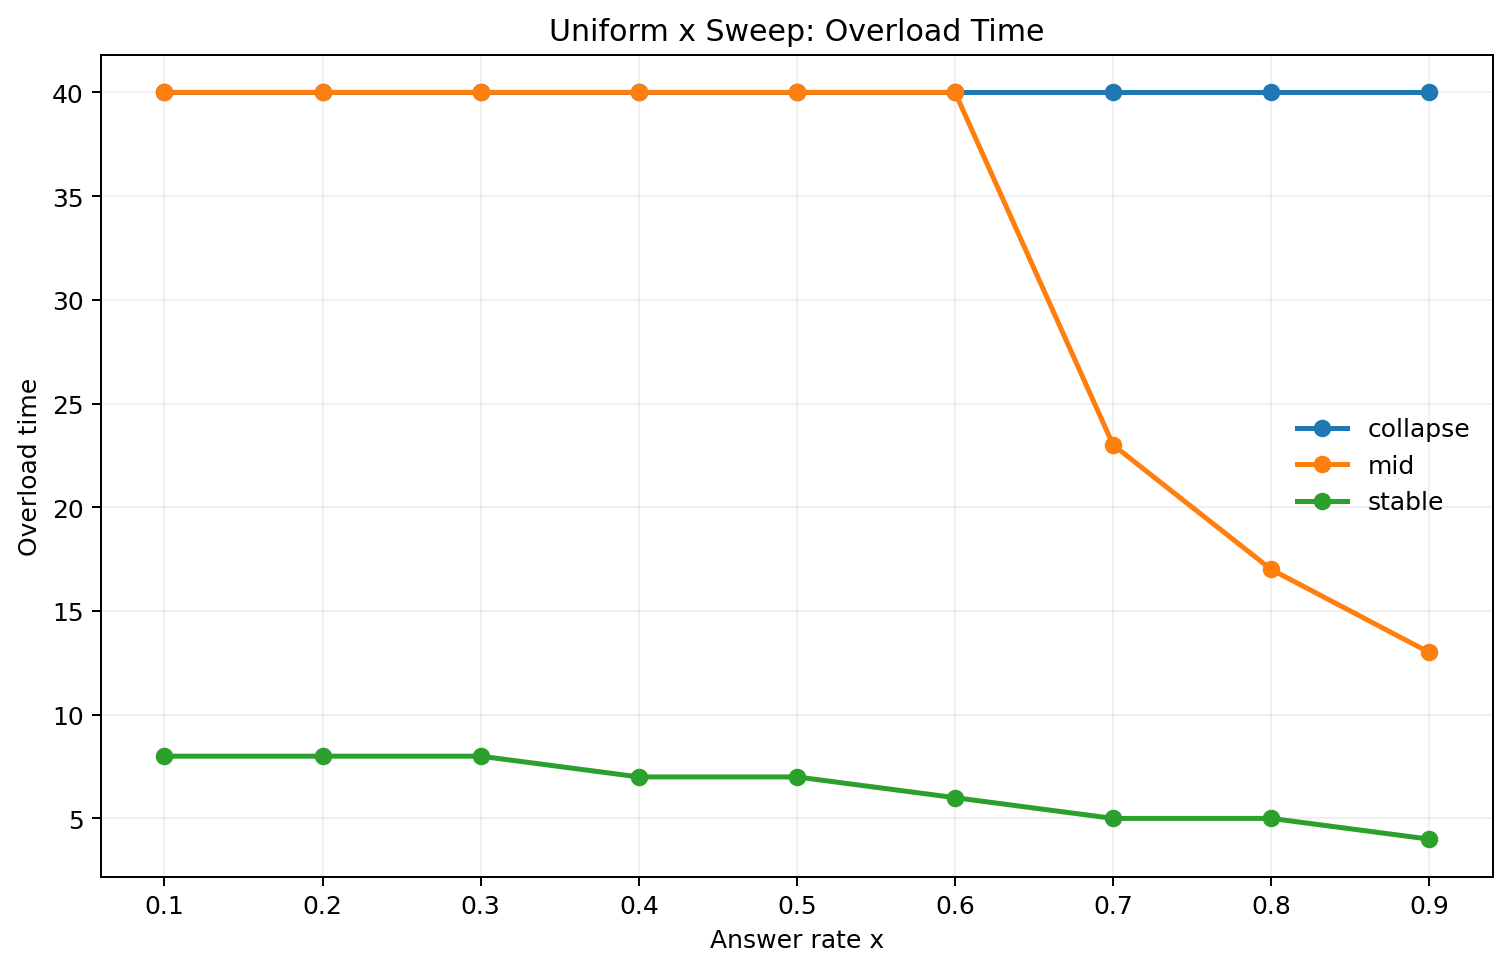
\includegraphics[width=0.48\textwidth]{../sim/figs/extra/x_sweep_overload.png}
\caption{$x$ sweep across the stable, mid, and collapse regimes. The same increase in response rate does not have the same effect in all regimes, which is one reason the system shows non-monotonic behavior.}
\end{figure}

\begin{figure}[H]
\centering
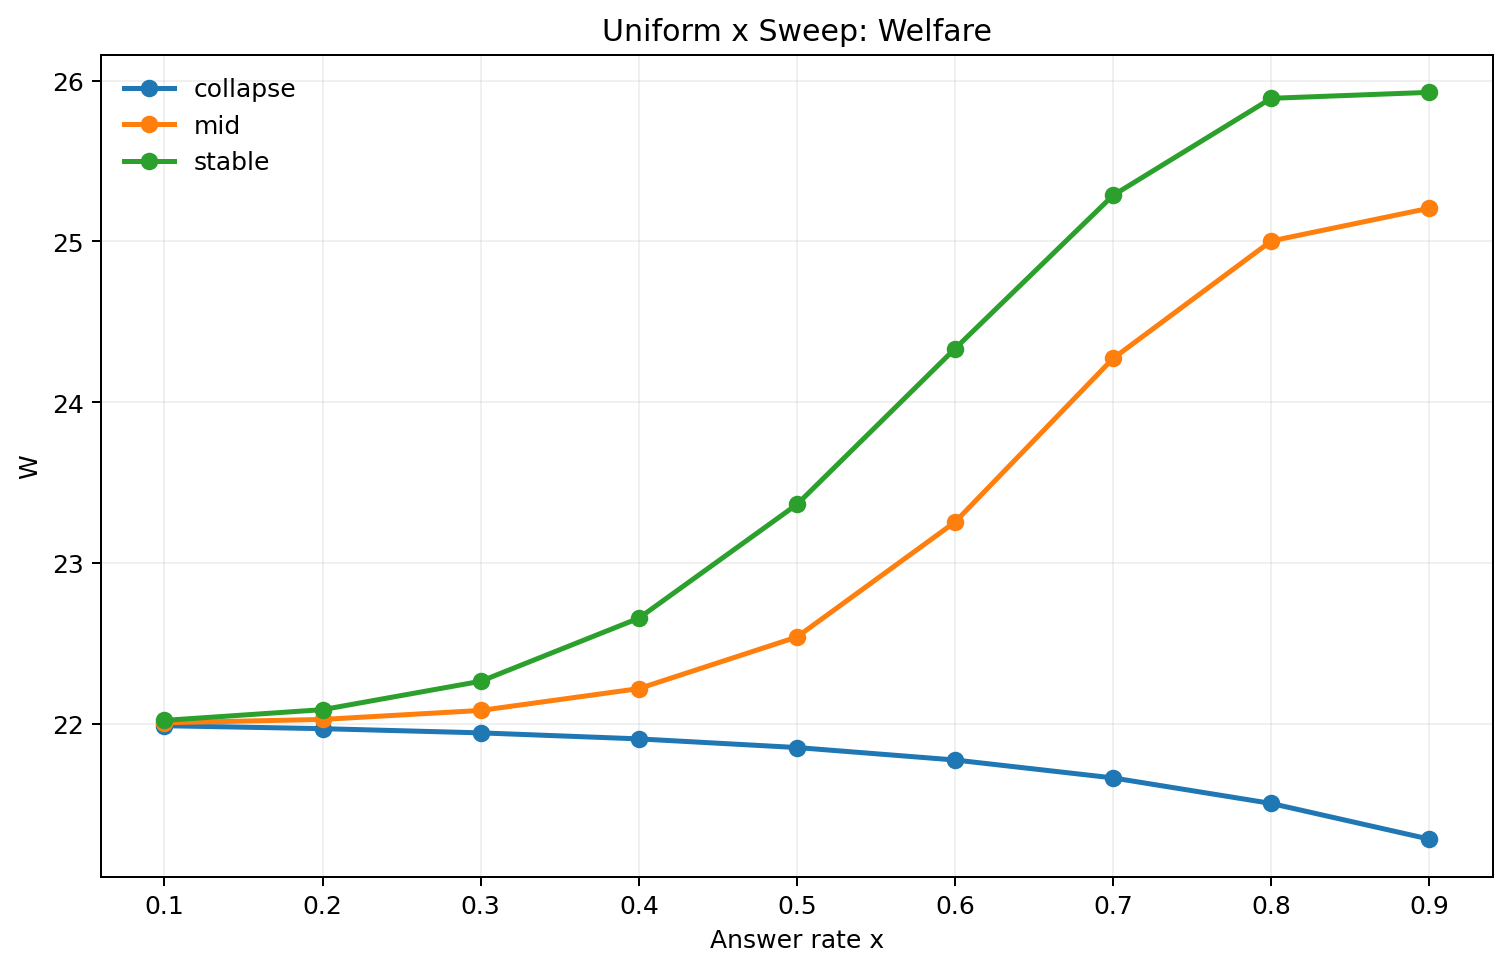
\includegraphics[width=0.48\textwidth]{../sim/figs/extra/x_sweep_welfare.png}
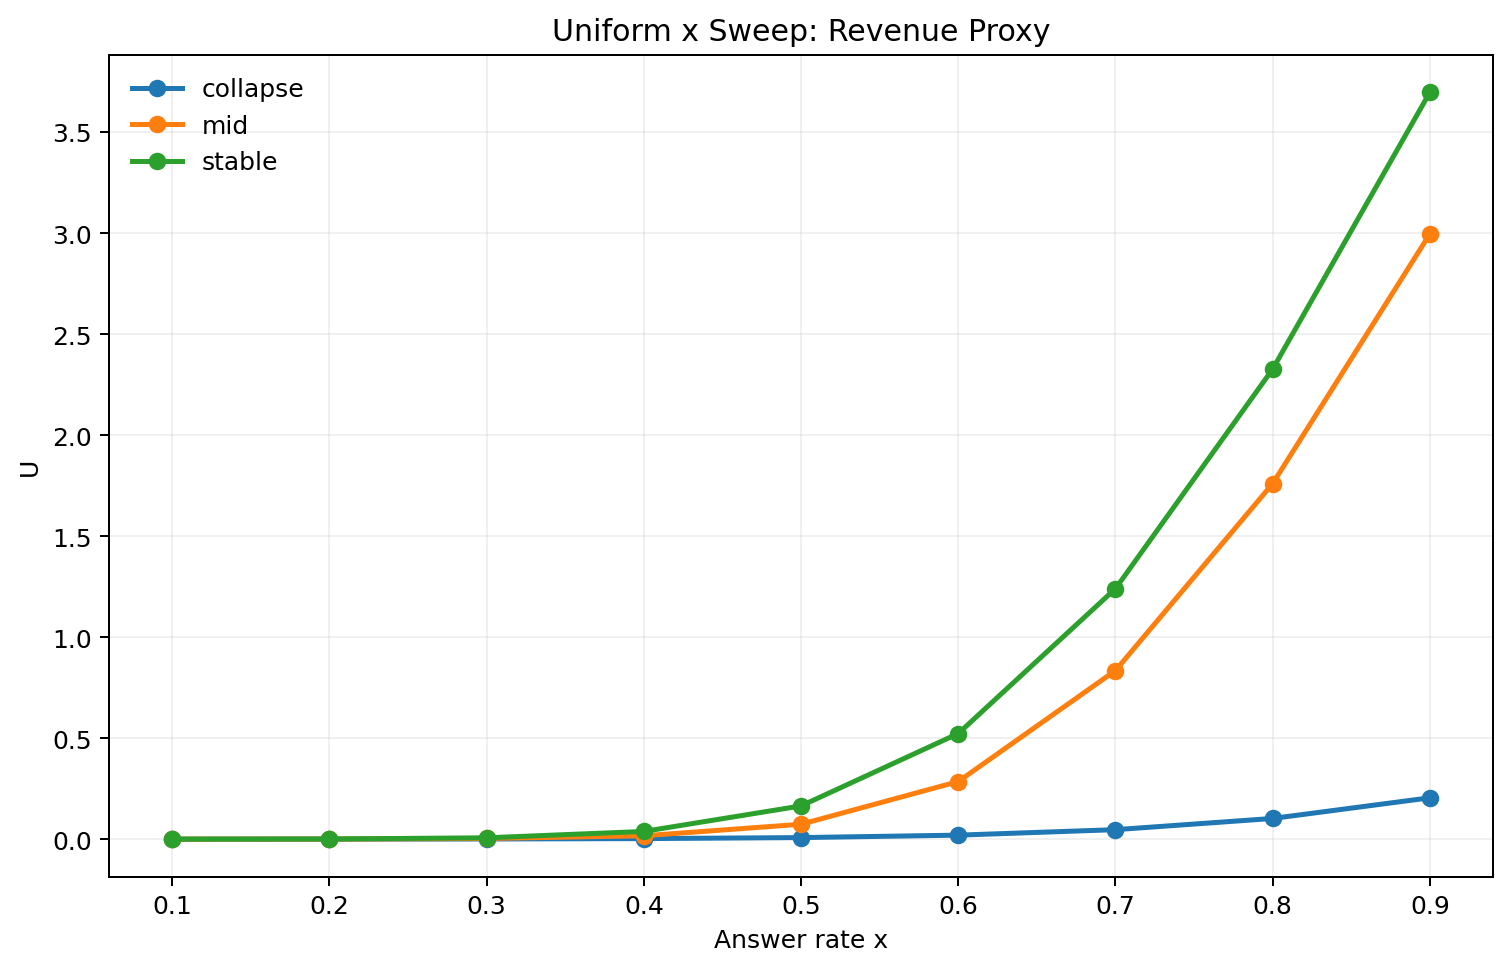
\includegraphics[width=0.48\textwidth]{../sim/figs/extra/x_sweep_revenue.png}
\caption{Welfare and revenue proxies across the $x$ sweep. These plots show that learning, overload, and short-run utility do not all peak at the same response level.}
\end{figure}

\begin{figure}[H]
\centering
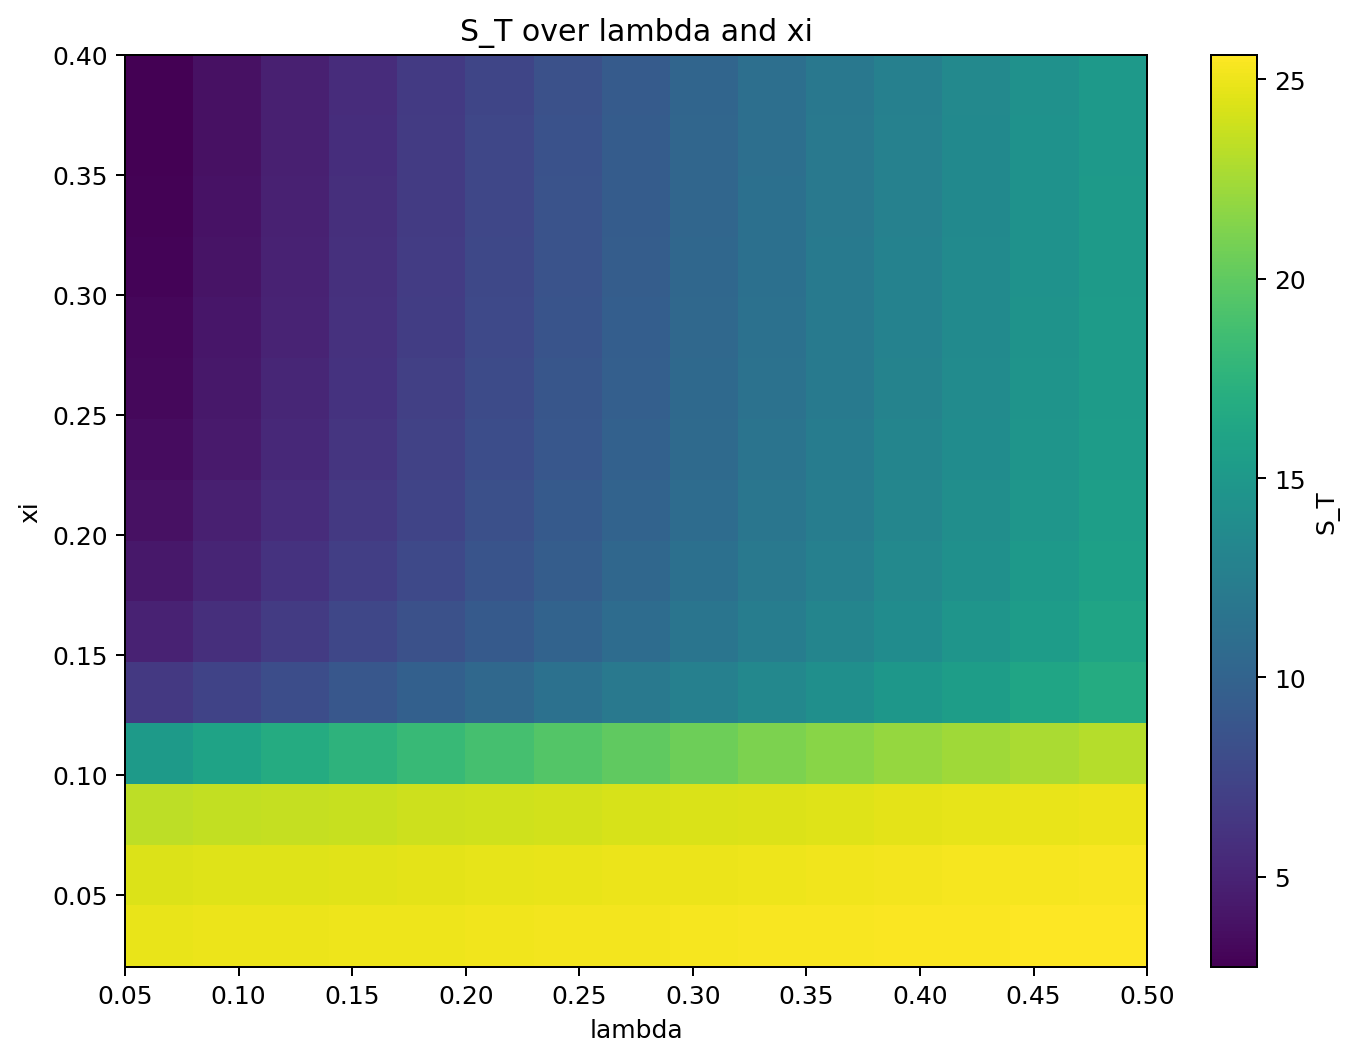
\includegraphics[width=0.48\textwidth]{../sim/figs/extra/heatmap_lambda_xi_ST.png}
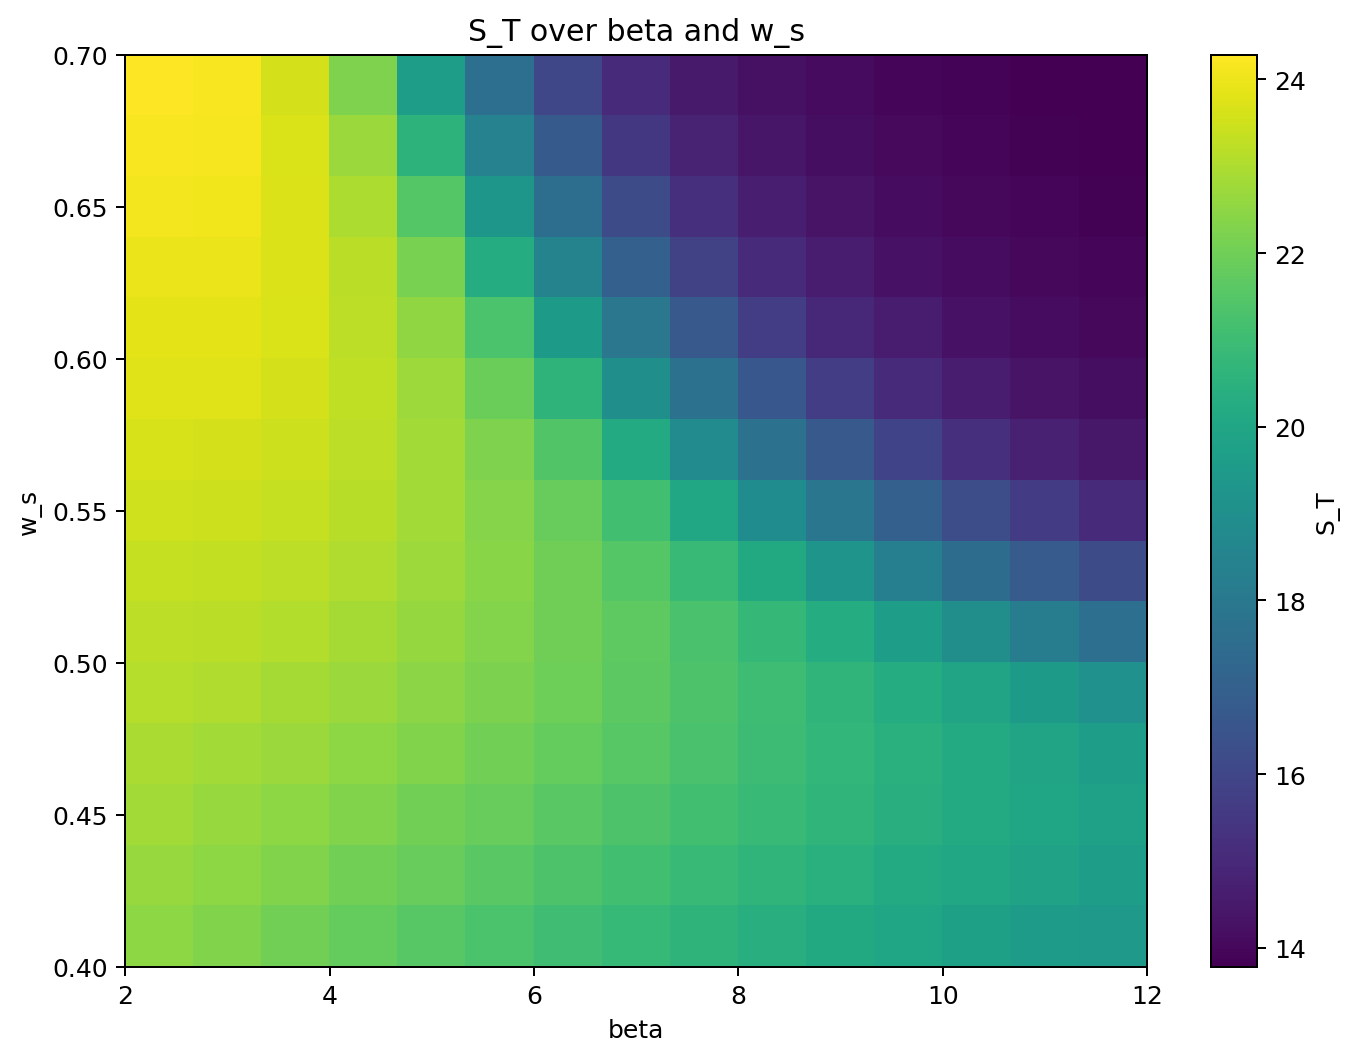
\includegraphics[width=0.48\textwidth]{../sim/figs/extra/heatmap_beta_ws_ST.png}
\caption{Additional phase diagrams. Left: variation over $(\lambda,\xi)$. Right: variation over $(\beta,w_s)$. These sweeps show where tipping becomes sharpest within the reduced-form simulator.}
\end{figure}

\begin{figure}[H]
\centering
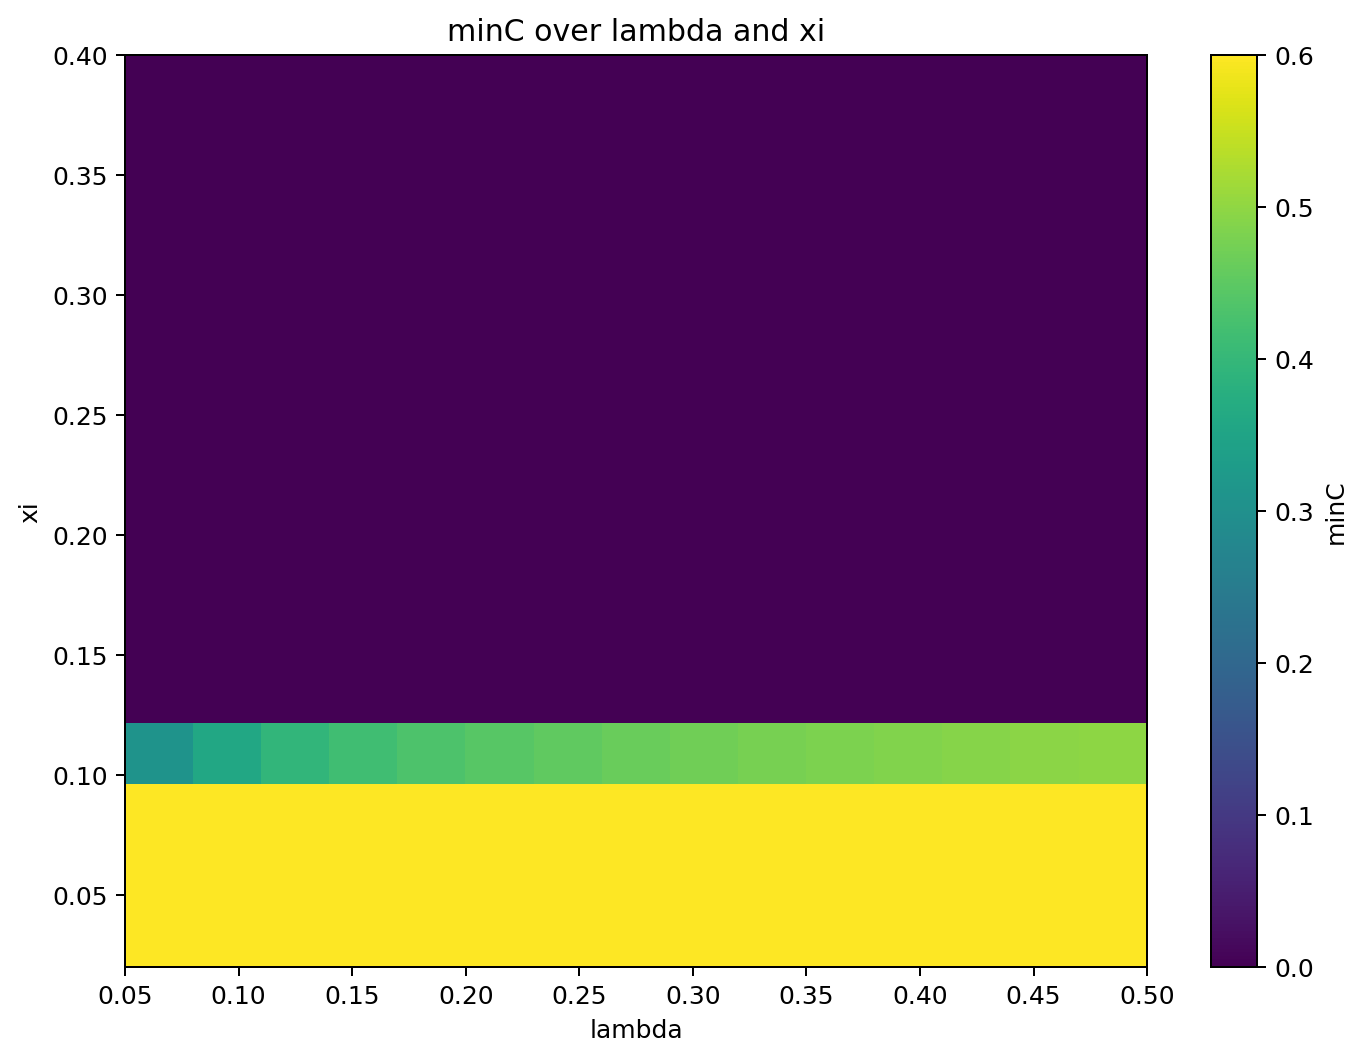
\includegraphics[width=0.48\textwidth]{../sim/figs/extra/heatmap_lambda_xi_minC.png}
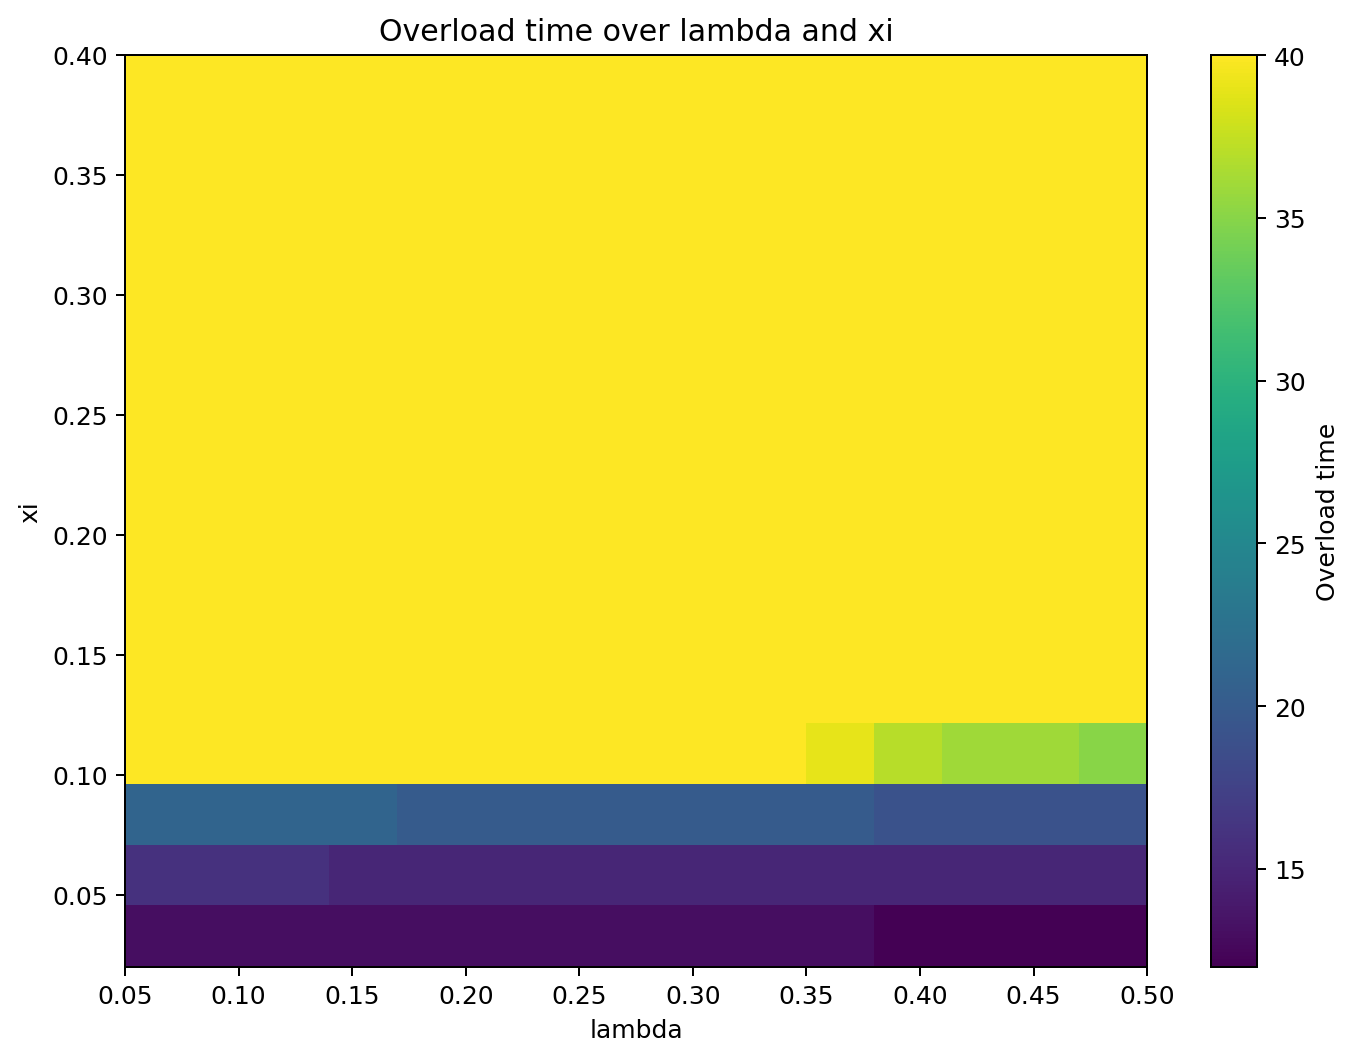
\includegraphics[width=0.48\textwidth]{../sim/figs/extra/heatmap_lambda_xi_overload.png}
\caption{Additional $(\lambda,\xi)$ views. Minimum capacity and overload time reveal the same tipping region from a different angle.}
\end{figure}

\begin{figure}[H]
\centering
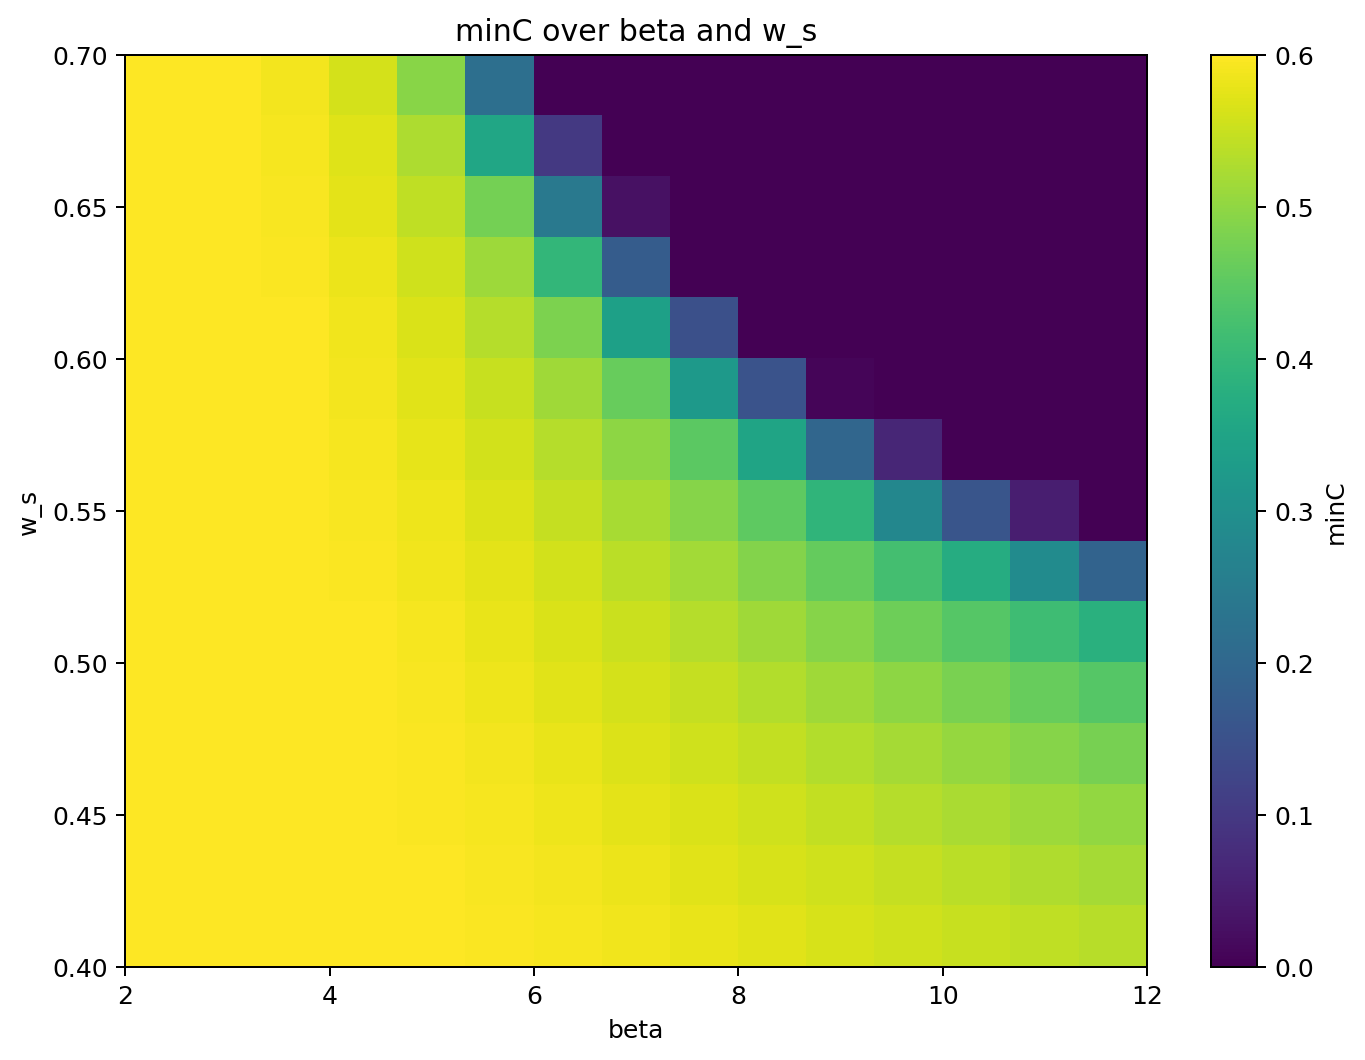
\includegraphics[width=0.48\textwidth]{../sim/figs/extra/heatmap_beta_ws_minC.png}
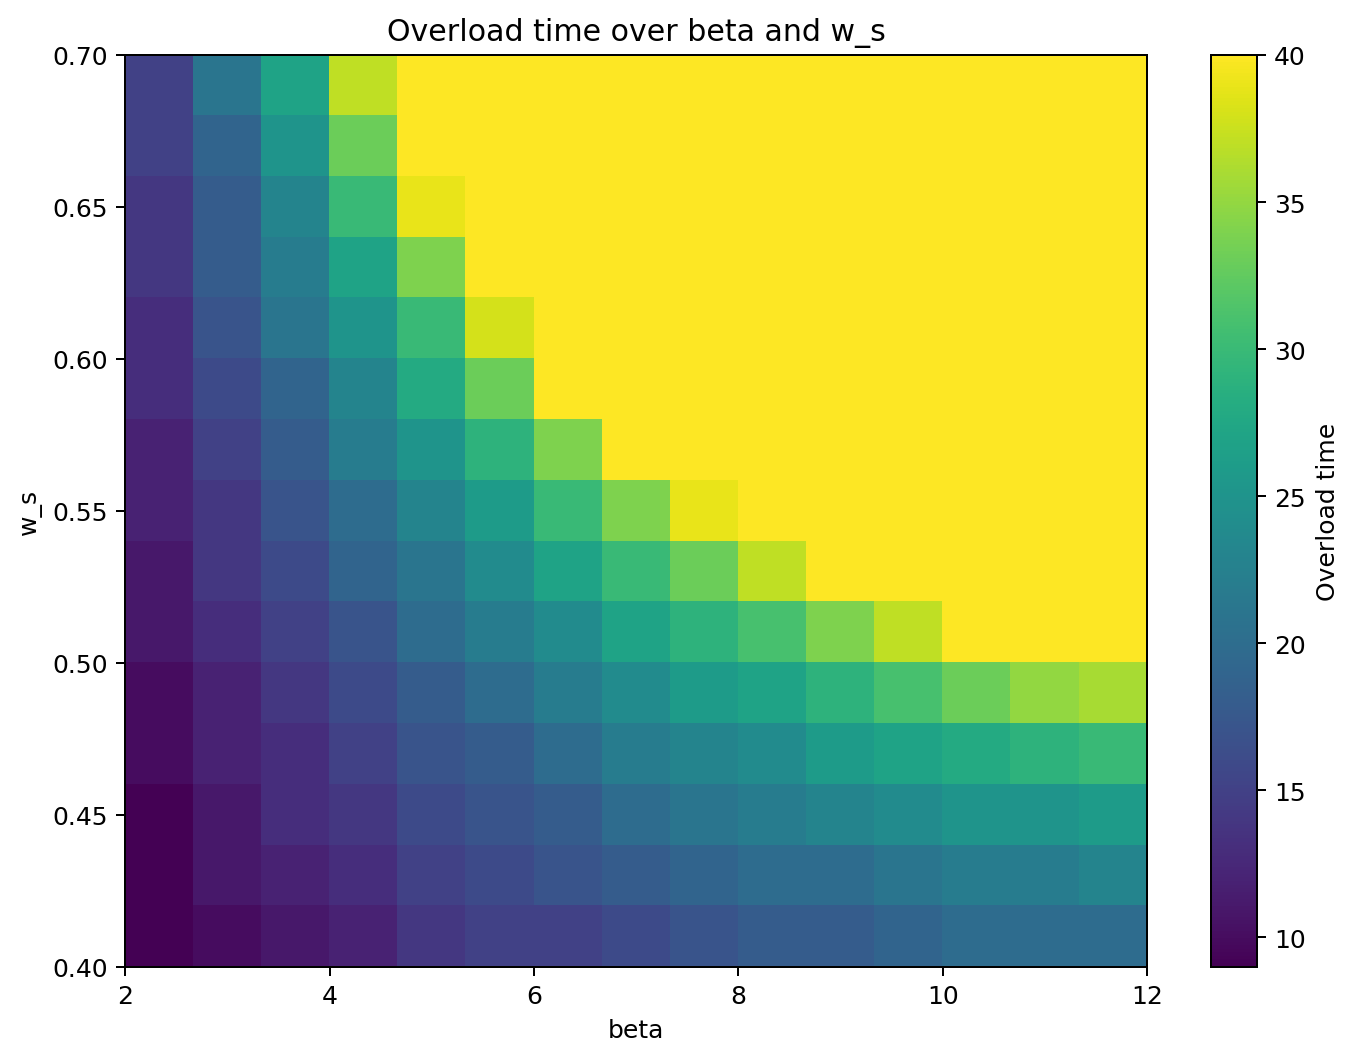
\includegraphics[width=0.48\textwidth]{../sim/figs/extra/heatmap_beta_ws_overload.png}
\caption{Additional $(\beta,w_s)$ views. User choice sensitivity and forum utility jointly affect how aggressively the system moves toward overload.}
\end{figure}

\begin{figure}[H]
\centering
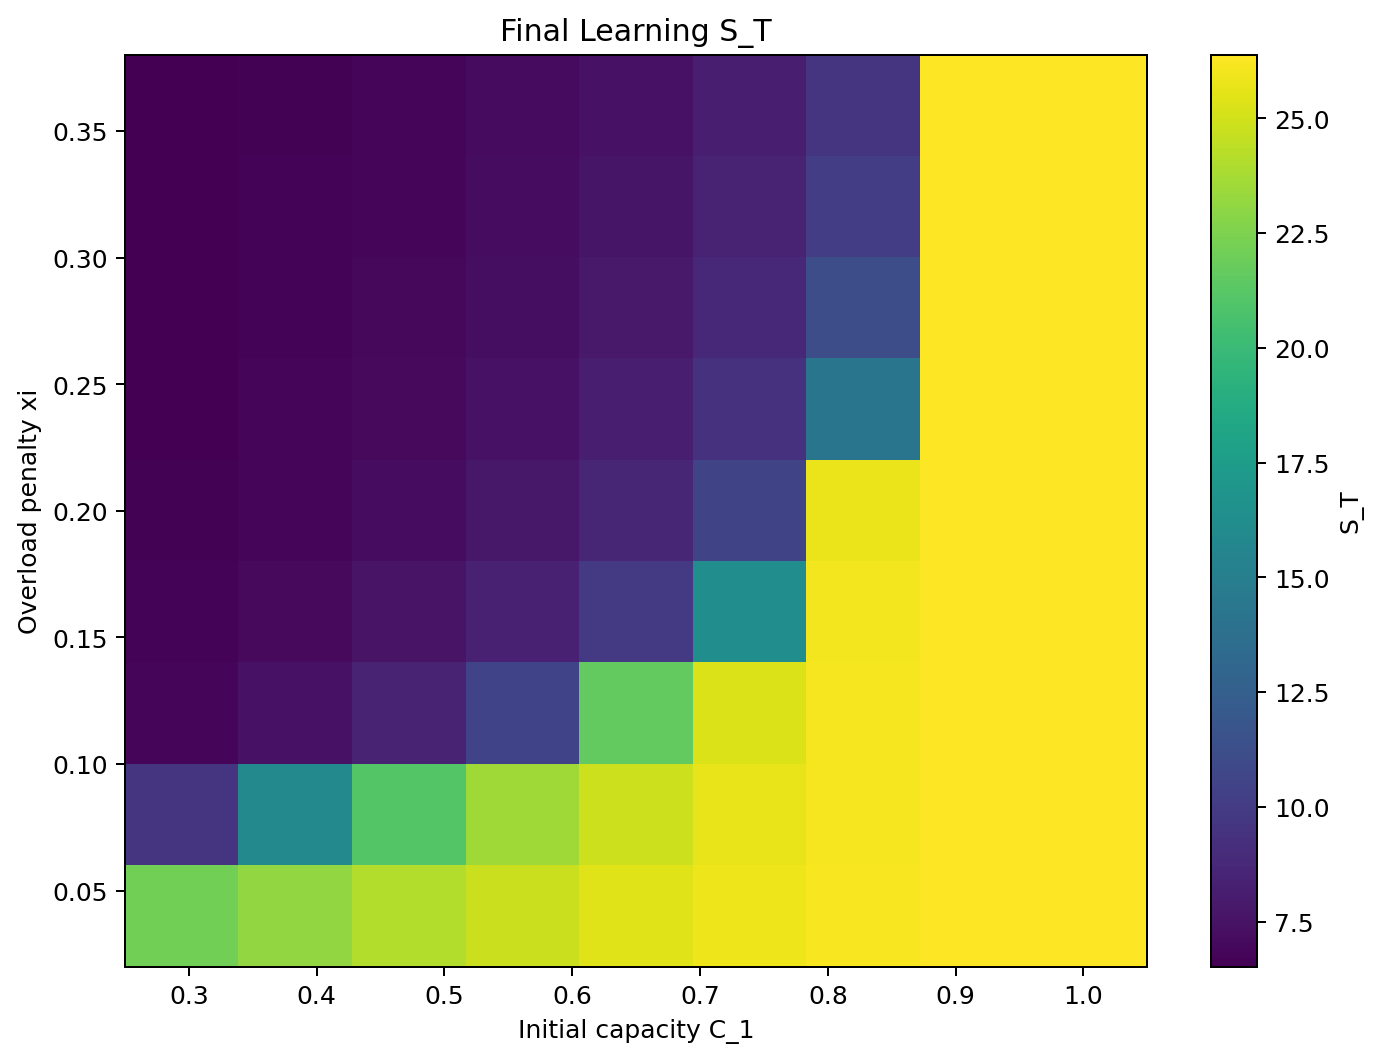
\includegraphics[width=0.48\textwidth]{../sim/figs/heatmap_ST.png}
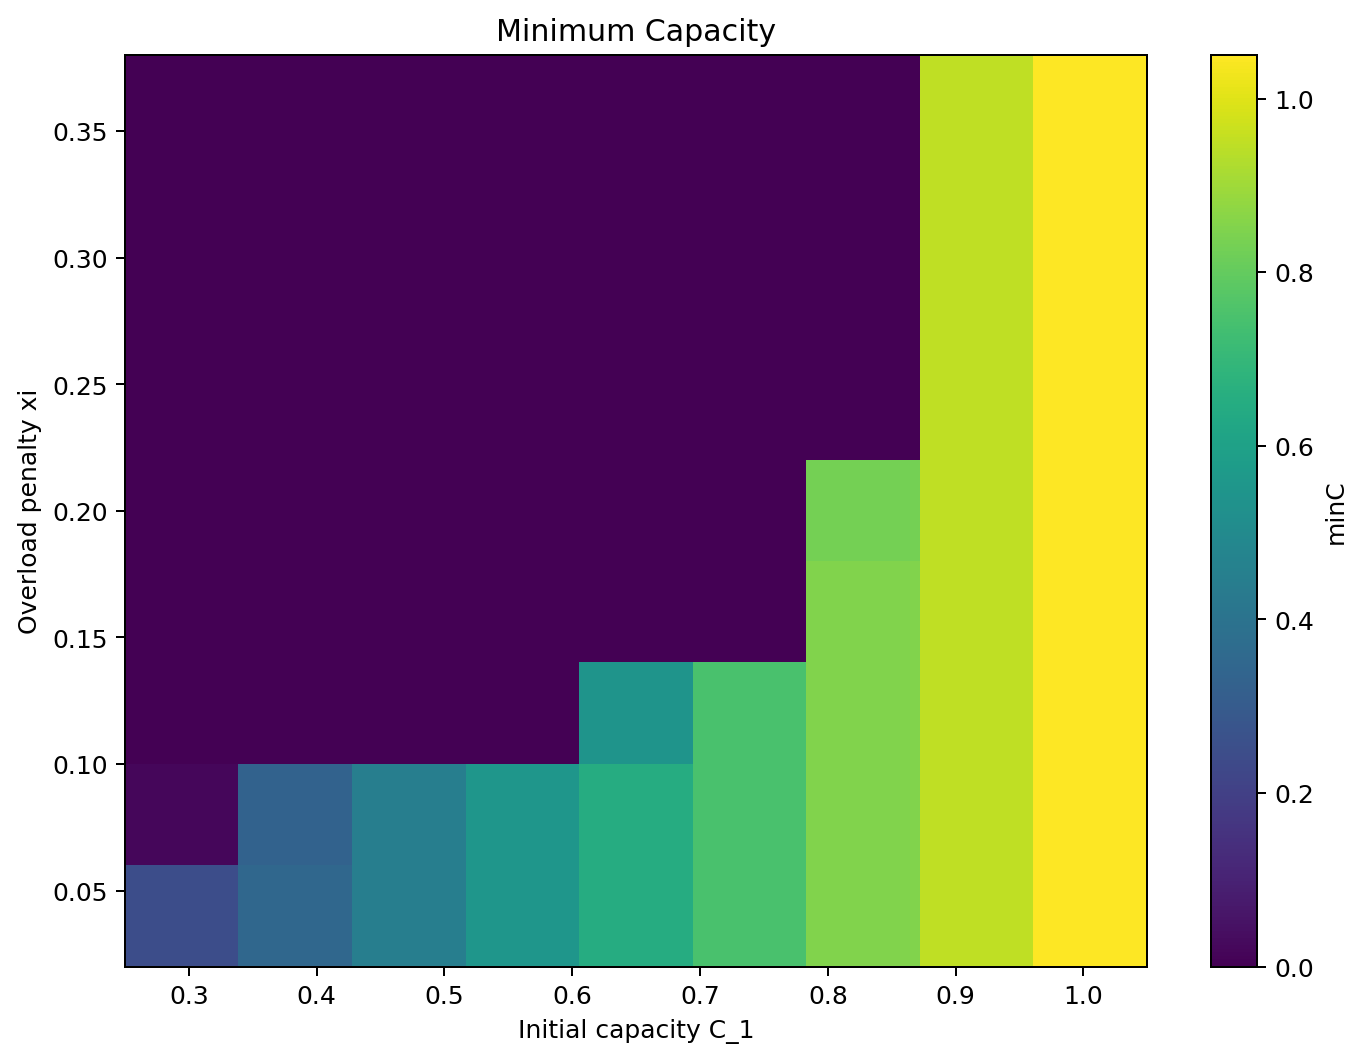
\includegraphics[width=0.48\textwidth]{../sim/figs/heatmap_minC.png}
\caption{Original baseline phase diagrams from the first simulator run. These provide a compact overview before the richer extra sweeps.}
\end{figure}

\begin{figure}[H]
\centering
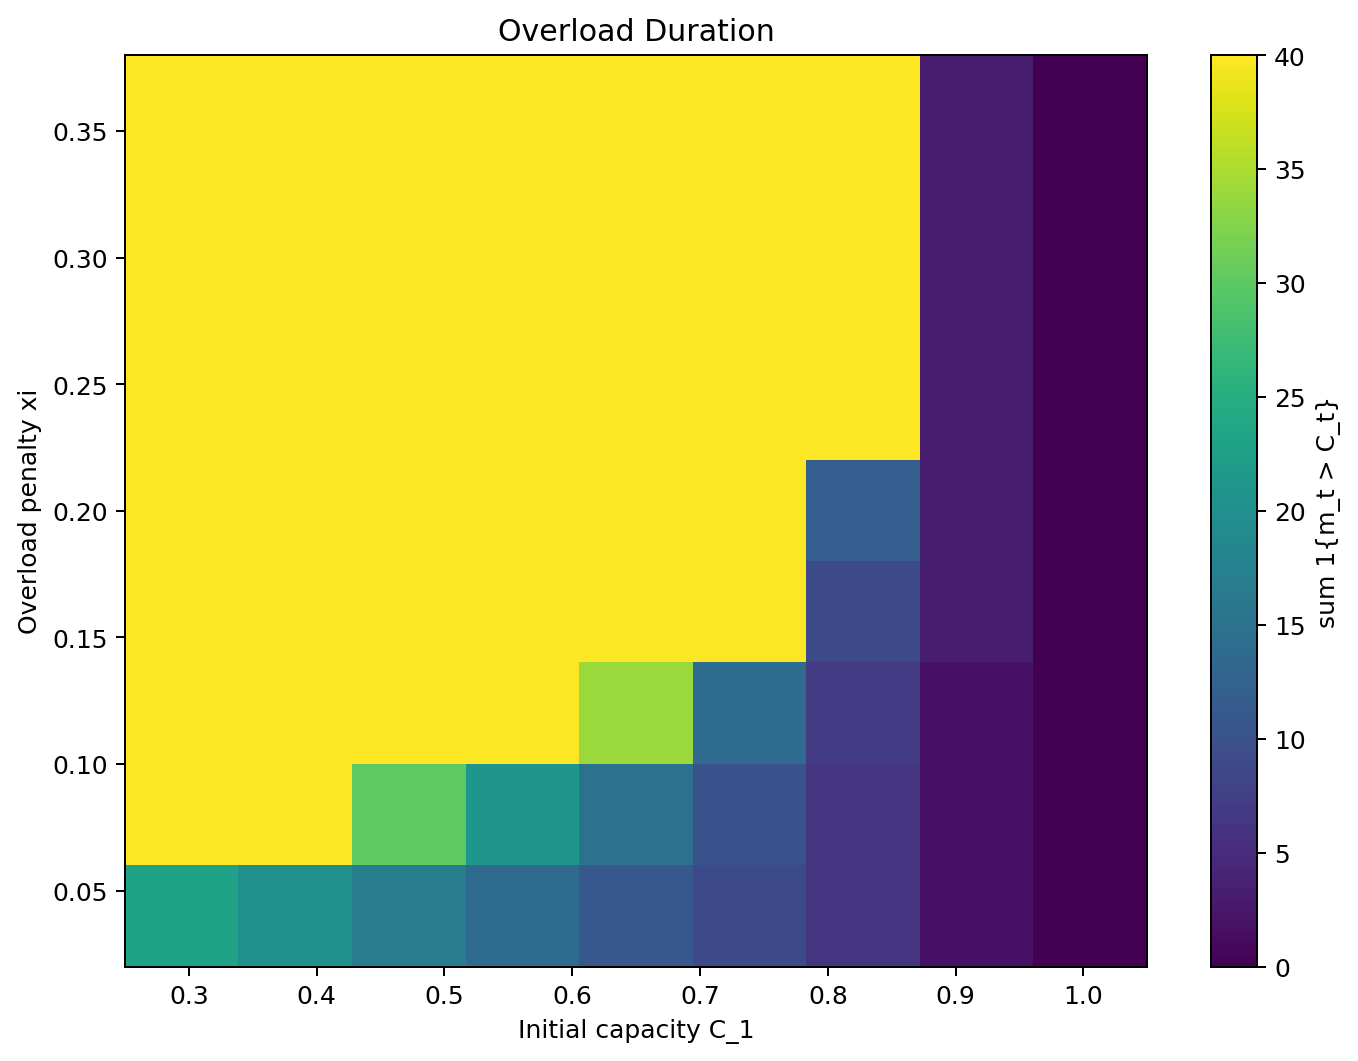
\includegraphics[width=0.48\textwidth]{../sim/figs/heatmap_overload.png}
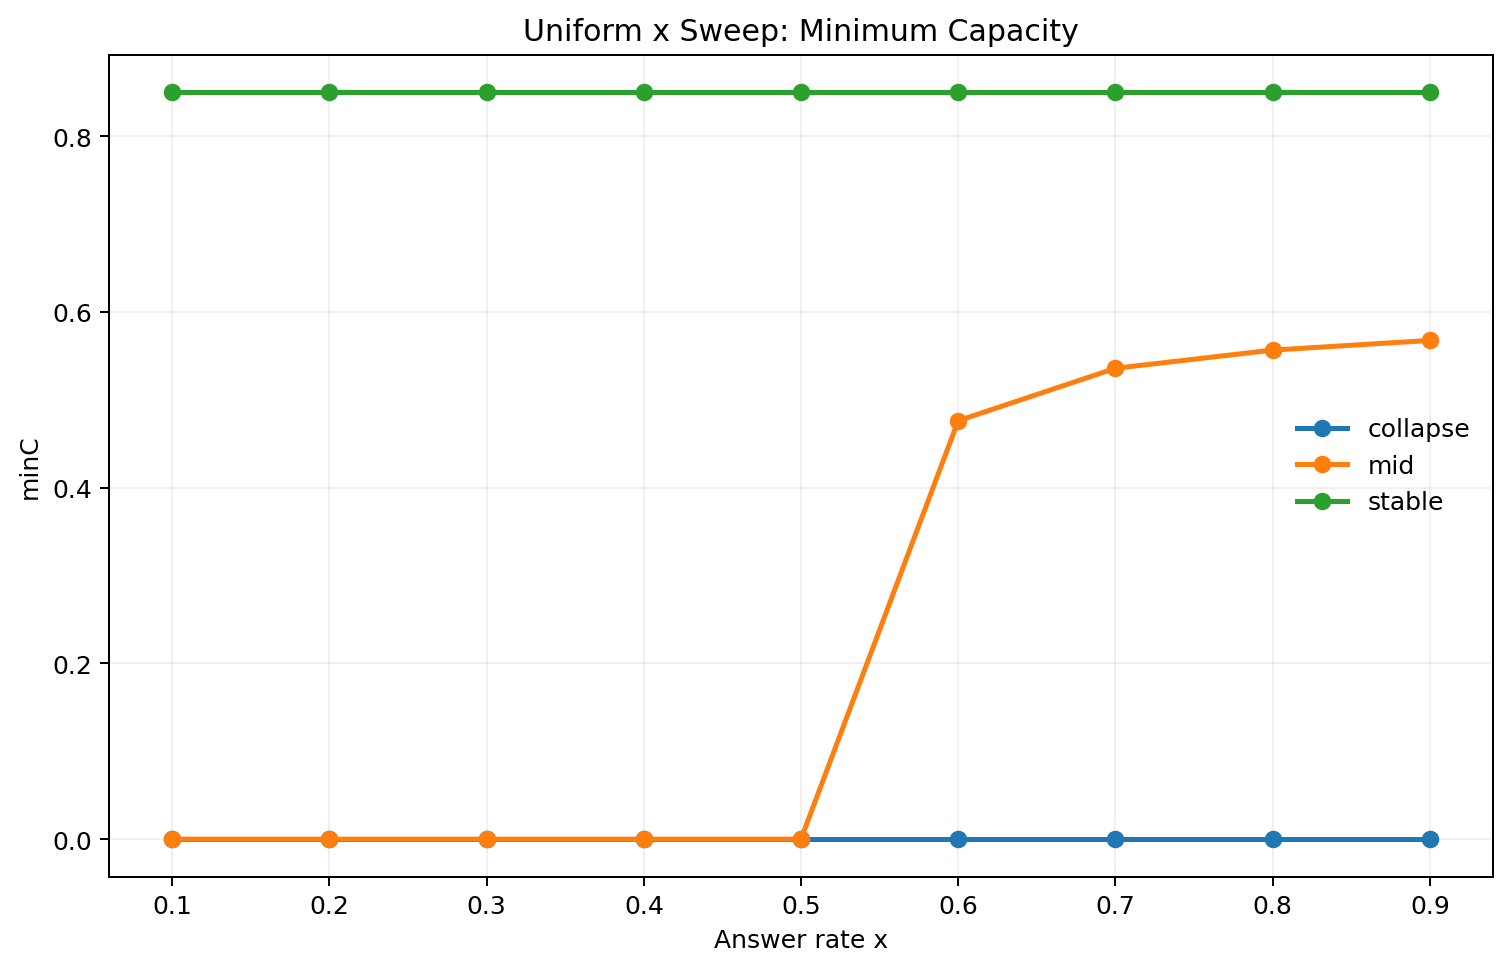
\includegraphics[width=0.48\textwidth]{../sim/figs/extra/x_sweep_minC.png}
\caption{Baseline overload map and the $x$-sweep minimum-capacity view. Together they show that both policy intensity and system parameters matter for forum health.}
\end{figure}

\section{Reproducibility}
The paper source is in \texttt{paper/main.tex}. Main commands used in this repository:
\begin{verbatim}
python sim/run_experiments.py --mode quick
python sim/run_experiments.py --mode full
\end{verbatim}

The manuscript uses pre-generated figures from \texttt{sim/figs/} and tabular results from \texttt{sim/results/}. The most important paper-facing files are:
\begin{itemize}[leftmargin=1.5em]
\item \texttt{paper/main.tex} for the manuscript source,
\item \texttt{paper/refs.bib} for bibliography entries,
\item \texttt{sim/figs/} and \texttt{sim/figs/extra/} for embedded figures,
\item \texttt{sim/results/summary.md} and \texttt{sim/results/extra/summary\_extra.md} for human-readable experiment summaries.
\end{itemize}

Important result files:
\begin{itemize}[leftmargin=1.5em]
\item \texttt{sim/results/extra/seed\_robustness.csv}
\item \texttt{sim/results/extra/policy\_compare\_extended.csv}
\item \texttt{sim/results/extra/rho\_ablation.csv}
\item \texttt{sim/results/extra/matched\_answered\_compare.csv}
\item \texttt{sim/results/extra/collapse\_boundary\_c1\_xi.csv}
\item \texttt{sim/results/extra/summary\_extra.md}
\end{itemize}

\bibliographystyle{plainnat}
\bibliography{refs}

\end{document}
